\section{Test Cases}


\textbf{Sign up \& login}\\

\begin{table}[ht]
\centering
\begin{tabularx}{\textwidth}{|c|c|X|X|X|c|}
\hline
\textbf{TID} & \textbf{User Role} & \textbf{Scenario Description} & \textbf{Steps to Execute} & \textbf{Expected Result} & \textbf{Status} \\ \hline
1 & Unregistered User & Create User Account & 1.Fill in the necessary details with valid data \newline 2.Click signup & Creation of a new user account & Pass \\ \hline
\end{tabularx}
\caption{Create User Account}
\end{table}

\begin{figure}[h!]
    \centering
    \textbf{Actual Result}
    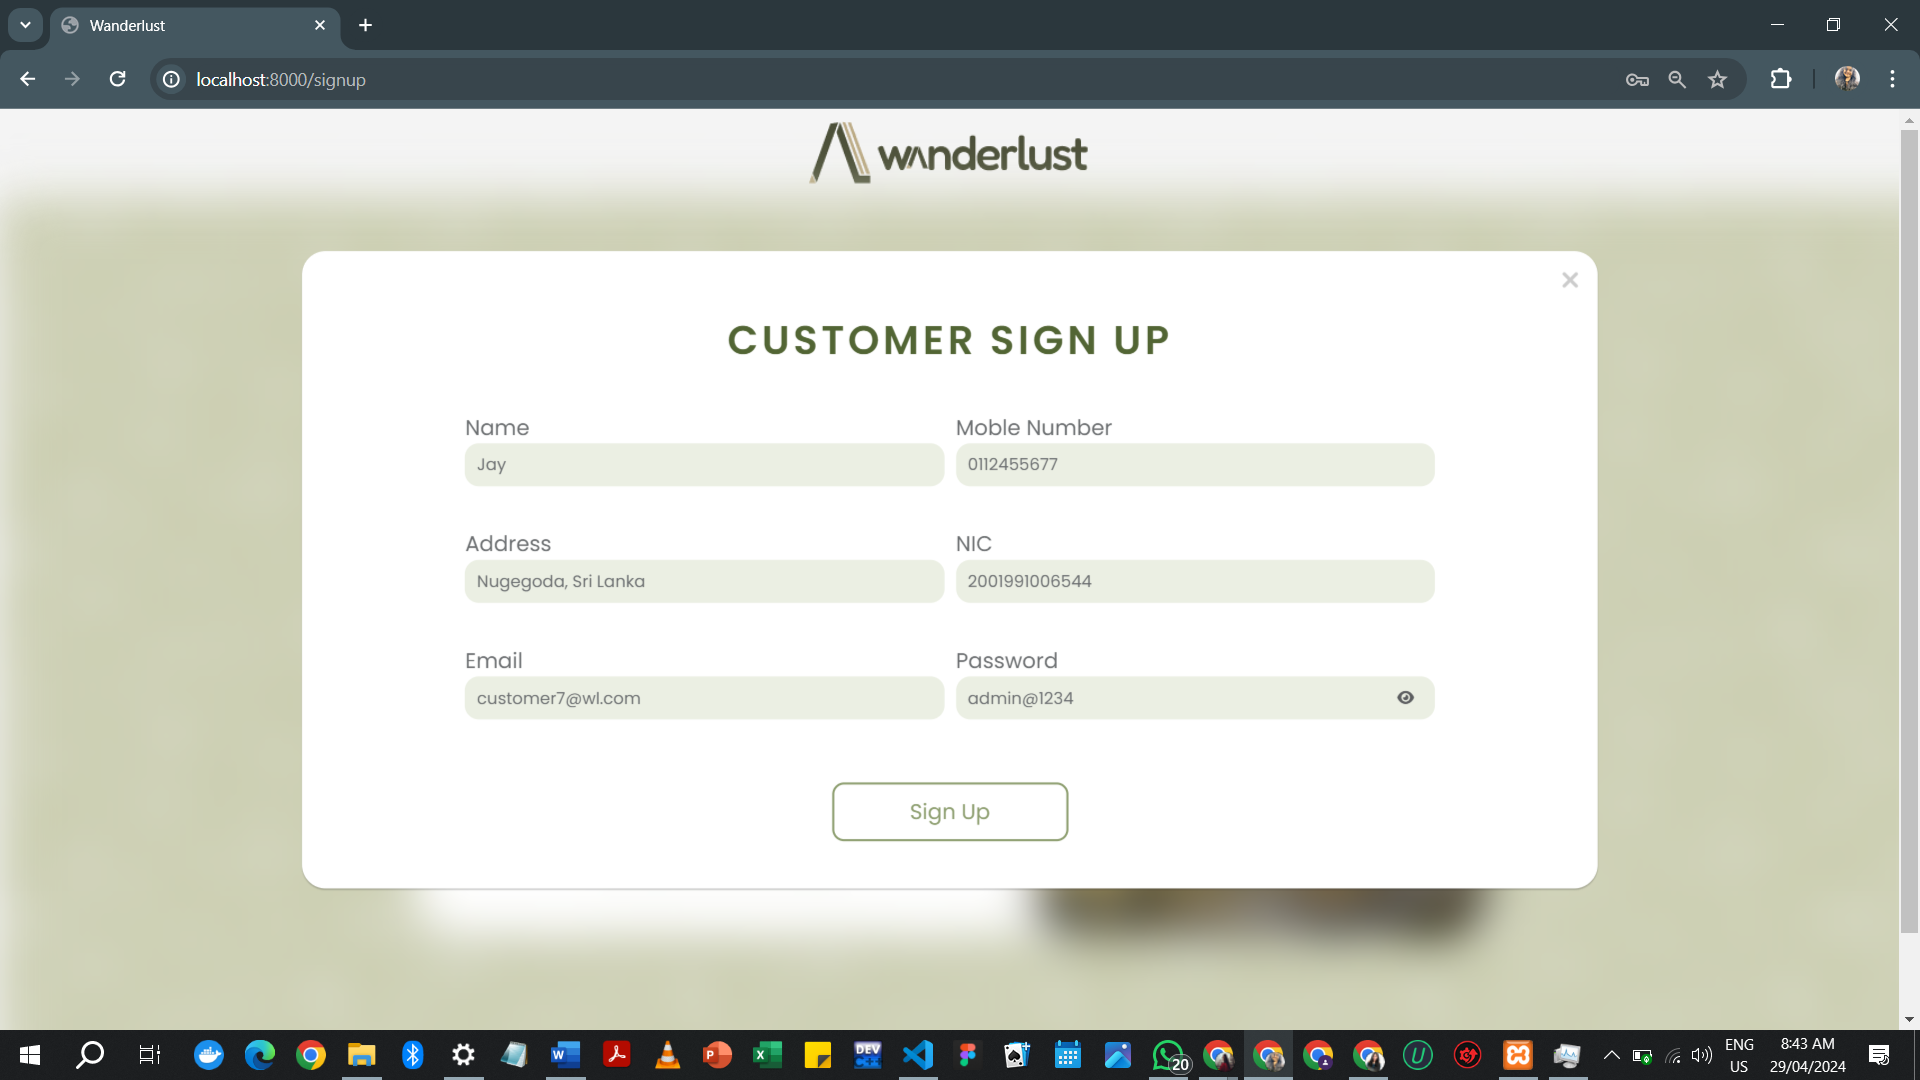
\includegraphics[width=1\textwidth]{Images/Test Cases/1.acc create cus.png}
\end{figure}



\begin{table}[ht]
\centering
\begin{tabularx}{\textwidth}{|c|c|X|X|X|c|}
\hline
\textbf{TID} & \textbf{User Role} & \textbf{Scenario Description} & \textbf{Steps to Execute} & \textbf{Expected Result} & \textbf{Status} \\ \hline
2 & Unregistered User & Create user account with invalid data & 1.Fill in the necessary details with invalid data \newline 2.Click signup & Not allowing to create a new user account & Pass \\ \hline
\end{tabularx}
\caption{Create User Account - Invalid Data}
\end{table}

\begin{figure}[h!]
    \centering
    \textbf{Actual Result}
    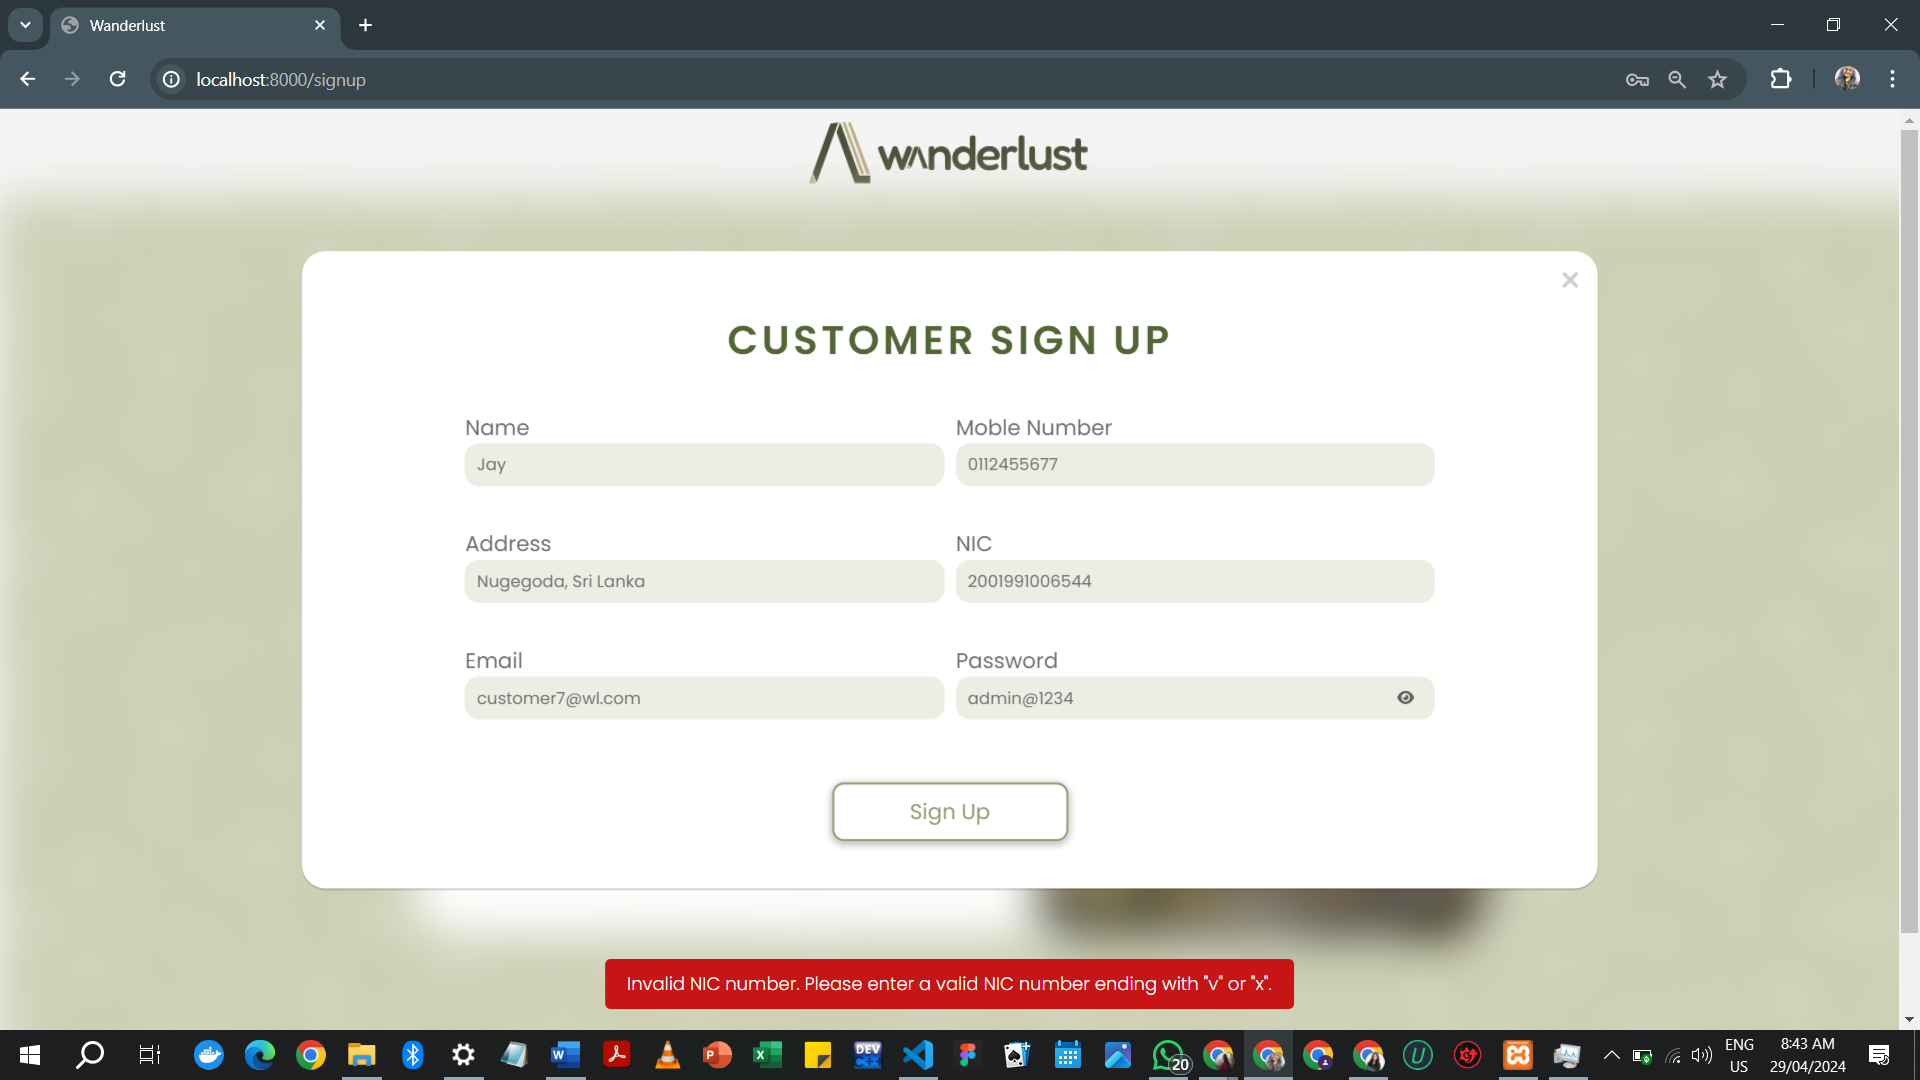
\includegraphics[width=1\textwidth]{Images/Test Cases/2. invalid acc create.png}
\end{figure}
\clearpage


\begin{table}[ht]
\centering
\begin{tabularx}{\textwidth}{|c|c|X|X|X|c|}
\hline
\textbf{TID} & \textbf{User Role} & \textbf{Scenario Description} & \textbf{Steps to Execute} & \textbf{Expected Result} & \textbf{Status} \\ \hline
3 & Customer & Login scenario with valid user & 1.Fill in the correct email address and the password \newline 2.Click login & Login to the account & Pass \\ \hline
\end{tabularx}
\caption{Login}
\end{table}

\begin{figure}[h!]
    \centering
    \textbf{Actual Result}
    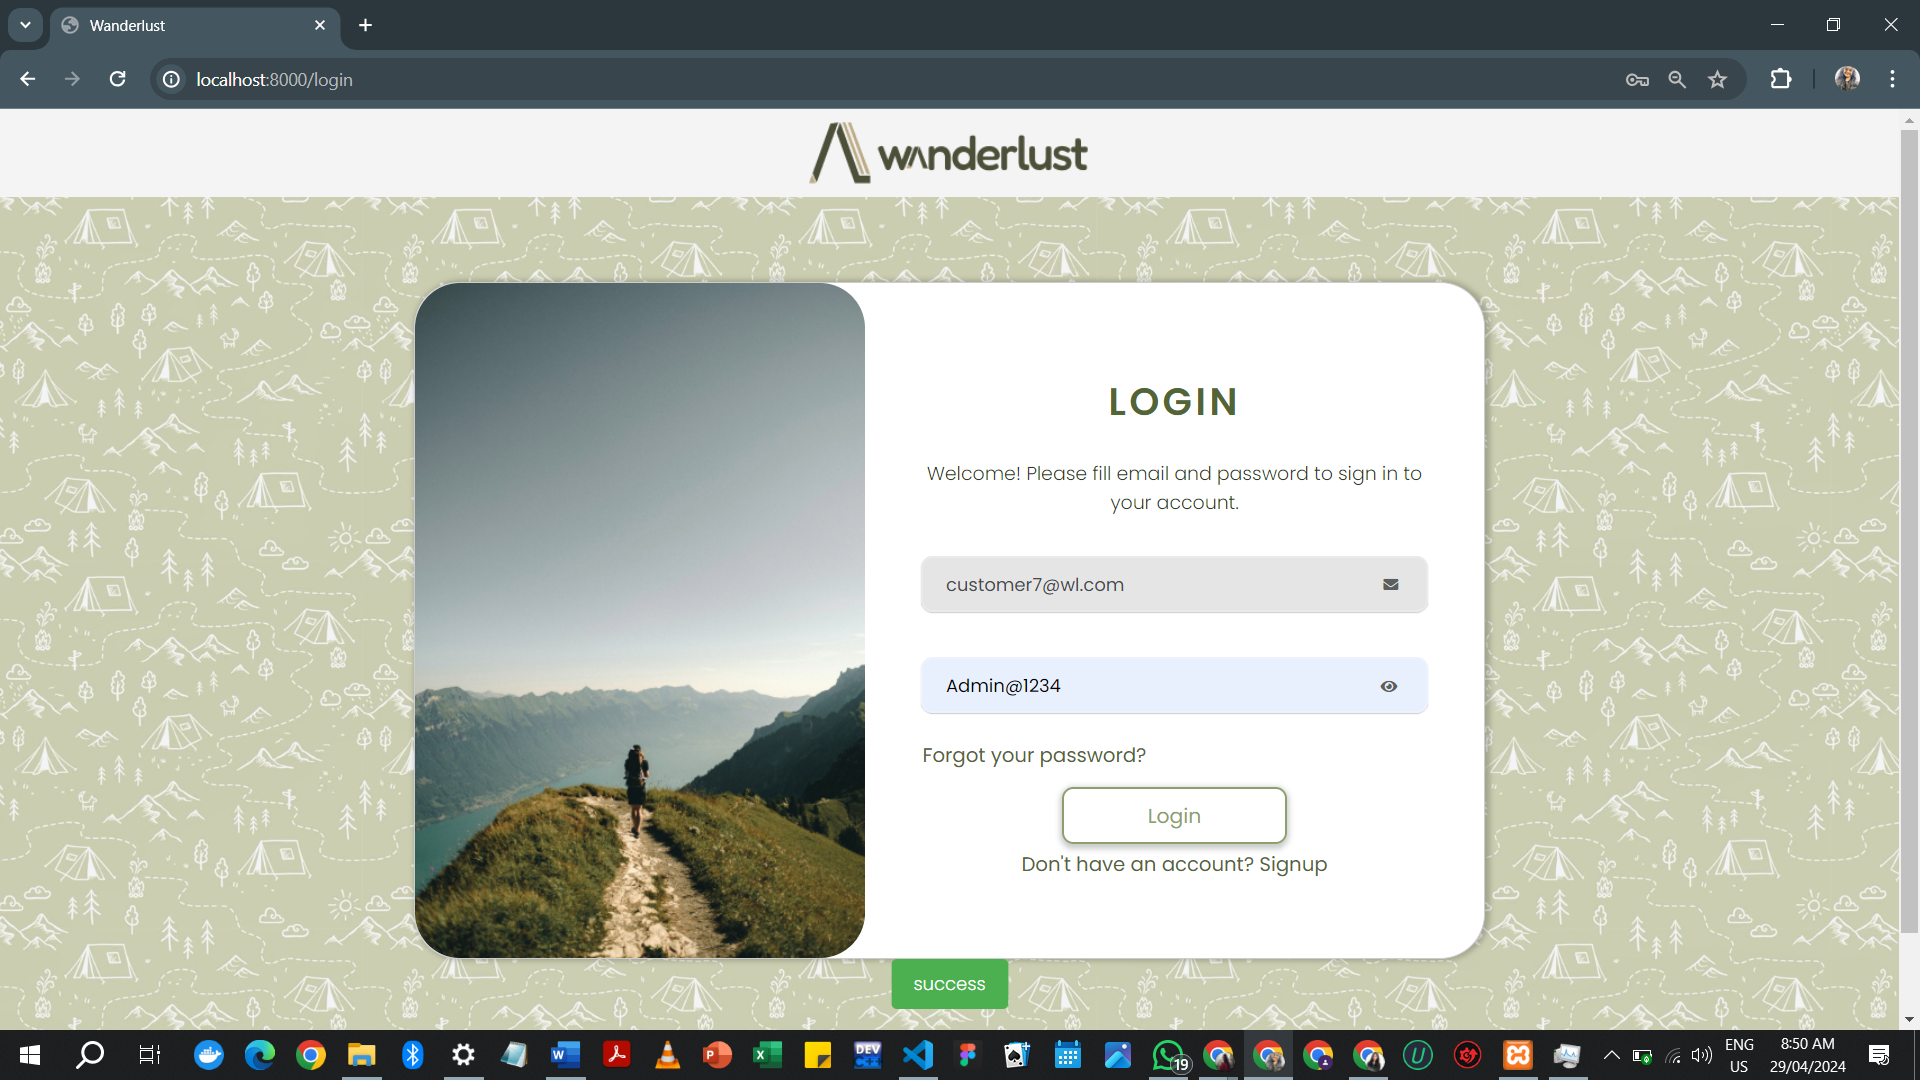
\includegraphics[width=1\textwidth]{Images/Test Cases/3. valid login.png}
\end{figure}
\clearpage


\begin{table}[ht]
\centering
\begin{tabularx}{\textwidth}{|c|c|X|X|X|c|}
\hline
\textbf{TID} & \textbf{User Role} & \textbf{Scenario Description} & \textbf{Steps to Execute} & \textbf{Expected Result} & \textbf{Status} \\ \hline
4 & Customer & Login scenario with valid user & 1.Fill in the correct email address and the password \newline 2.Click login & Login to the account & Pass \\ \hline
\end{tabularx}
\caption{Login with invalid Credentials}
\end{table}

\begin{figure}[h!]
    \centering
    \textbf{Actual Result}
    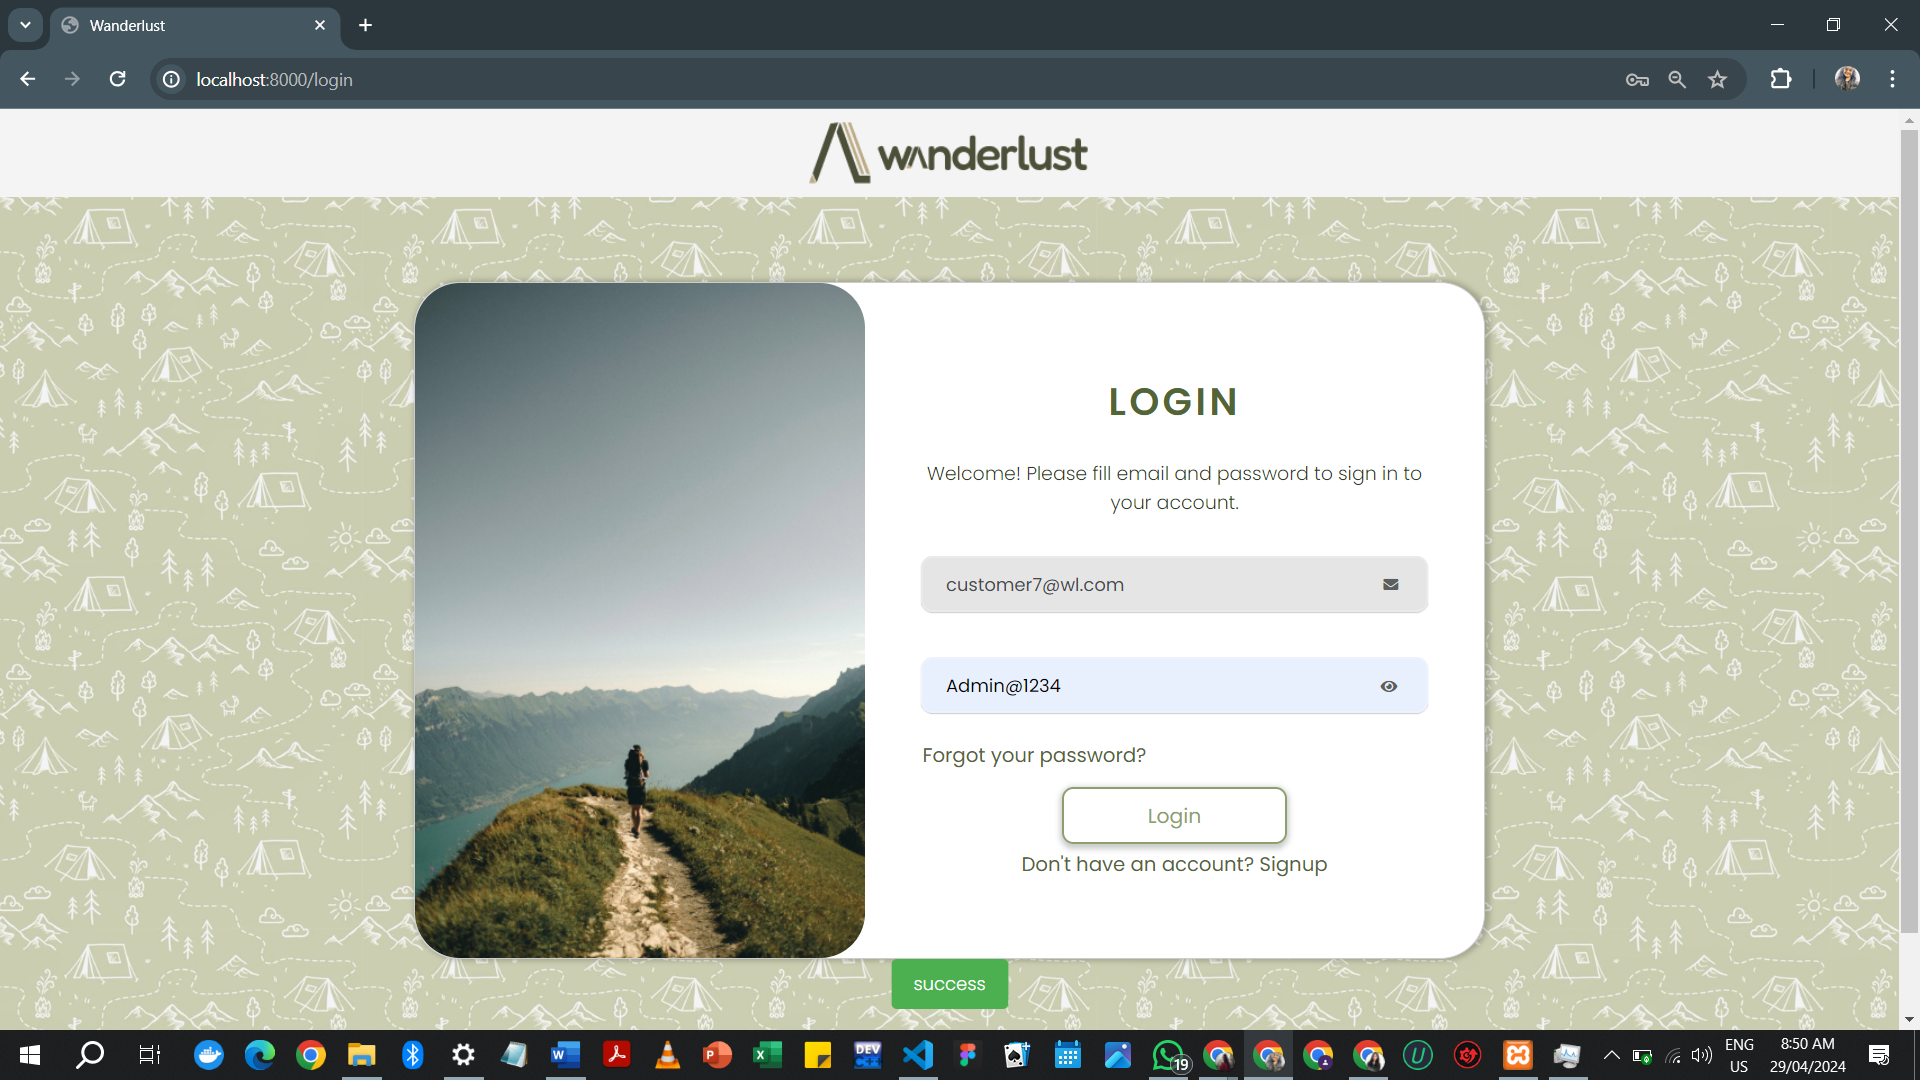
\includegraphics[width=1\textwidth]{Images/Test Cases/3. valid login.png}
\end{figure}
\clearpage



\textbf{Searching for Equipment}\\
\begin{table}[ht]
\centering
\begin{tabularx}{\textwidth}{|c|c|X|X|X|c|}
\hline
\textbf{TID} & \textbf{User Role} & \textbf{Scenario Description} & \textbf{Steps to Execute} & \textbf{Expected Result} & \textbf{Status} \\ \hline
5 & Customer & Selecting invalid time range for renting period & Selecting a time period of end date coming before the start date & Error message & Pass \\ \hline
\end{tabularx}
\caption{Equipment search with invalid time}
\end{table}

\begin{figure}[h!]
    \centering
    \textbf{Actual Result}
    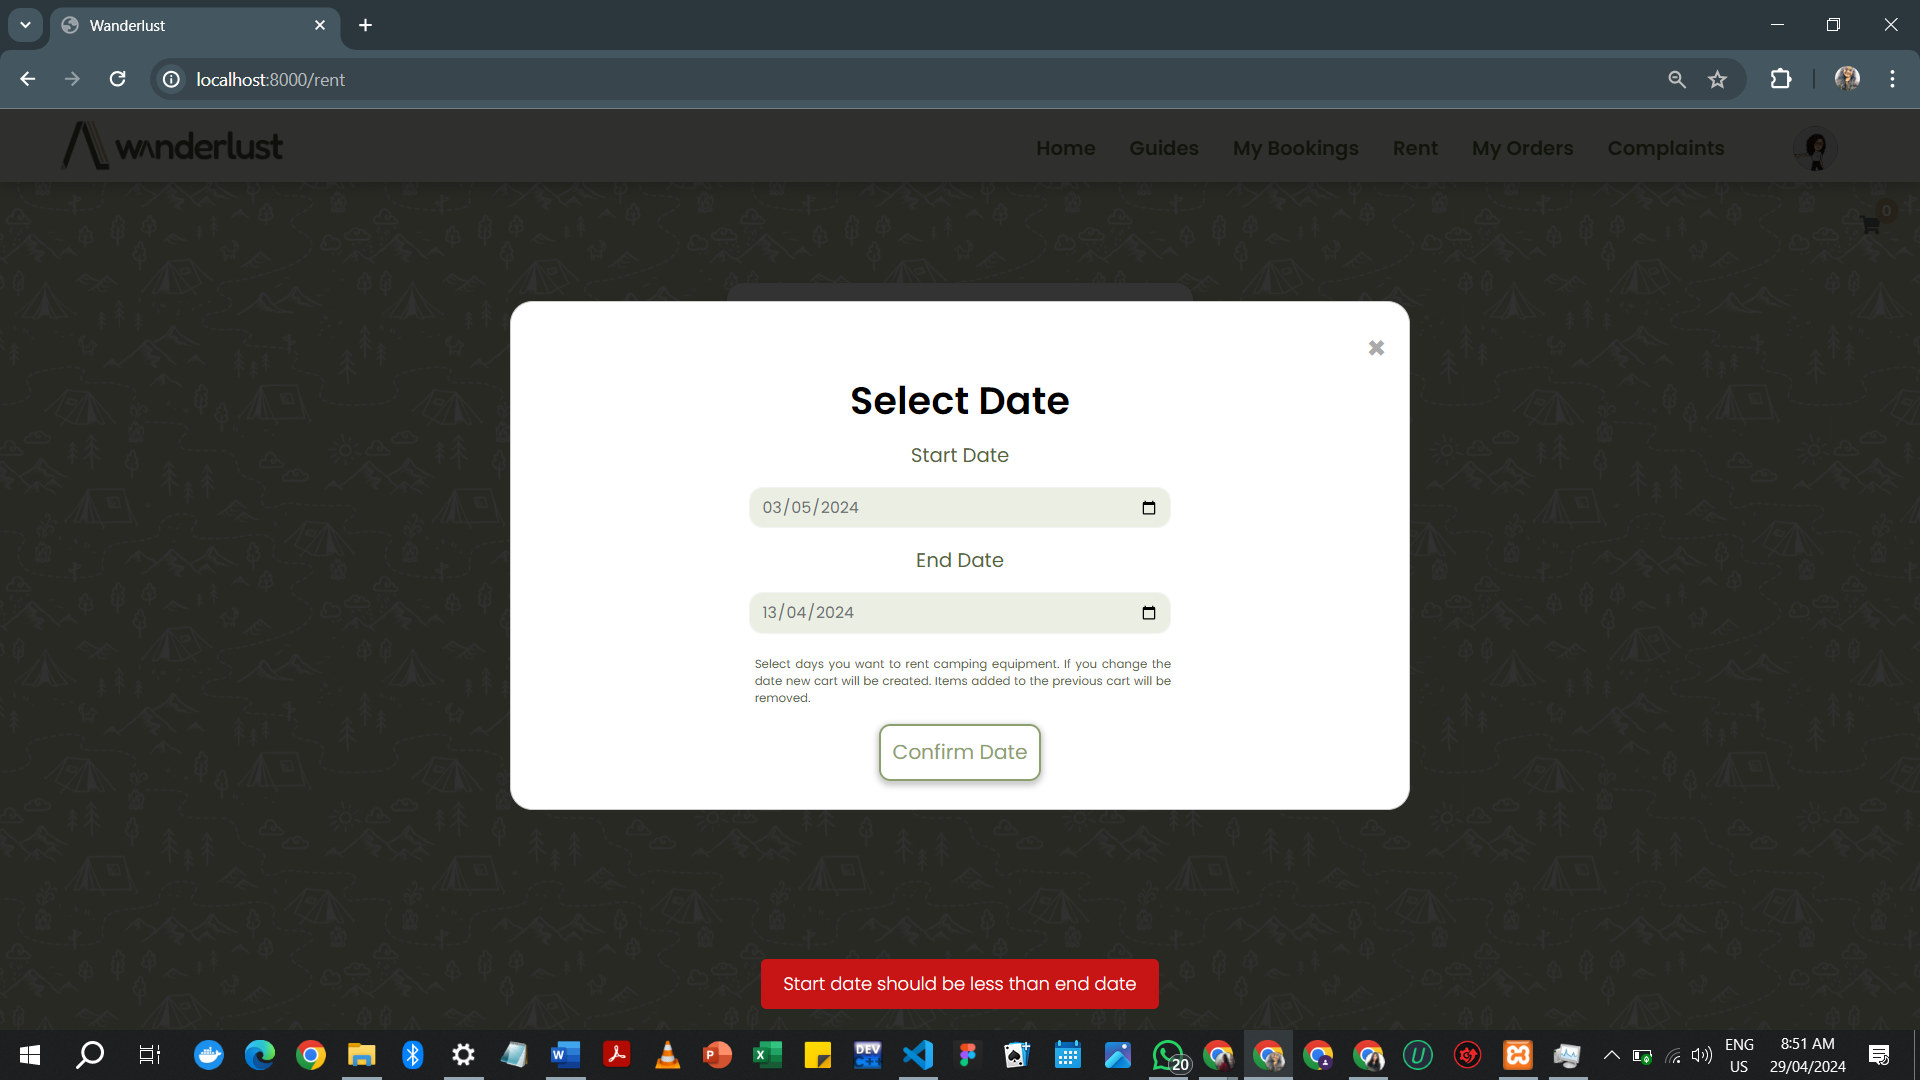
\includegraphics[width=1\textwidth]{Images/Test Cases/5. invalid time rent.png}
\end{figure}
\clearpage


\begin{table}[ht]
\centering
\begin{tabularx}{\textwidth}{|c|c|X|X|X|c|}
\hline
\textbf{TID} & \textbf{User Role} & \textbf{Scenario Description} & \textbf{Steps to Execute} & \textbf{Expected Result} & \textbf{Status} \\ \hline
6 & Customer & Invalid place for location & Selecting a place out of Sri Lankan borders & Error message & Pass \\ \hline
\end{tabularx}
\caption{Equipment search with invalid place}
\end{table}

\begin{figure}[h!]
    \centering
    \textbf{Actual Result}
    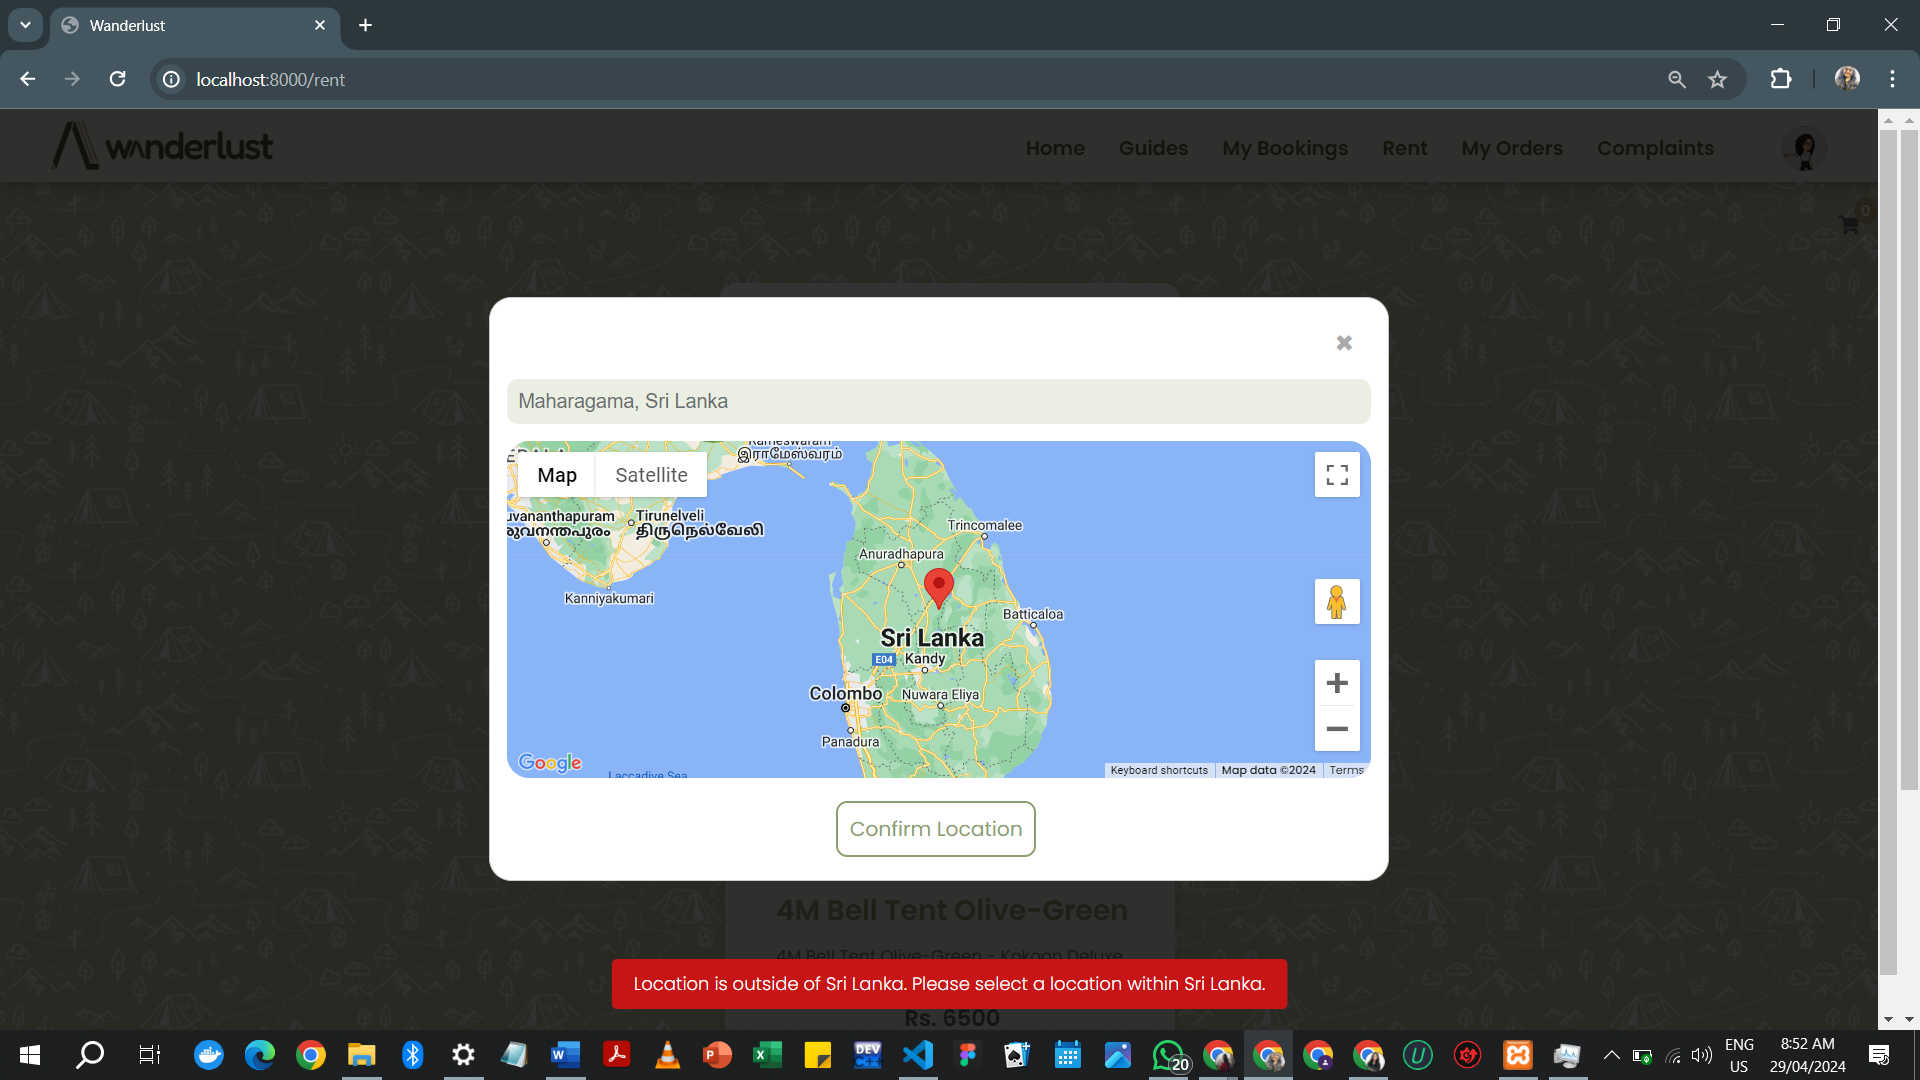
\includegraphics[width=1\textwidth]{Images/Test Cases/6. invalid place rent.png}
\end{figure}
\clearpage


\begin{table}[ht]
\centering
\begin{tabularx}{\textwidth}{|c|c|X|X|X|c|}
\hline
\textbf{TID} & \textbf{User Role} & \textbf{Scenario Description} & \textbf{Steps to Execute} & \textbf{Expected Result} & \textbf{Status} \\ \hline
7 & Customer & Equipment Search with valid inputs & 1.Fill in valid date, location and item name \newline 2.Click search & Available equipment & Pass \\ \hline
\end{tabularx}
\caption{Equipment search with valid details}
\end{table}

\begin{figure}[h!]
    \centering
    \textbf{Actual Result}
    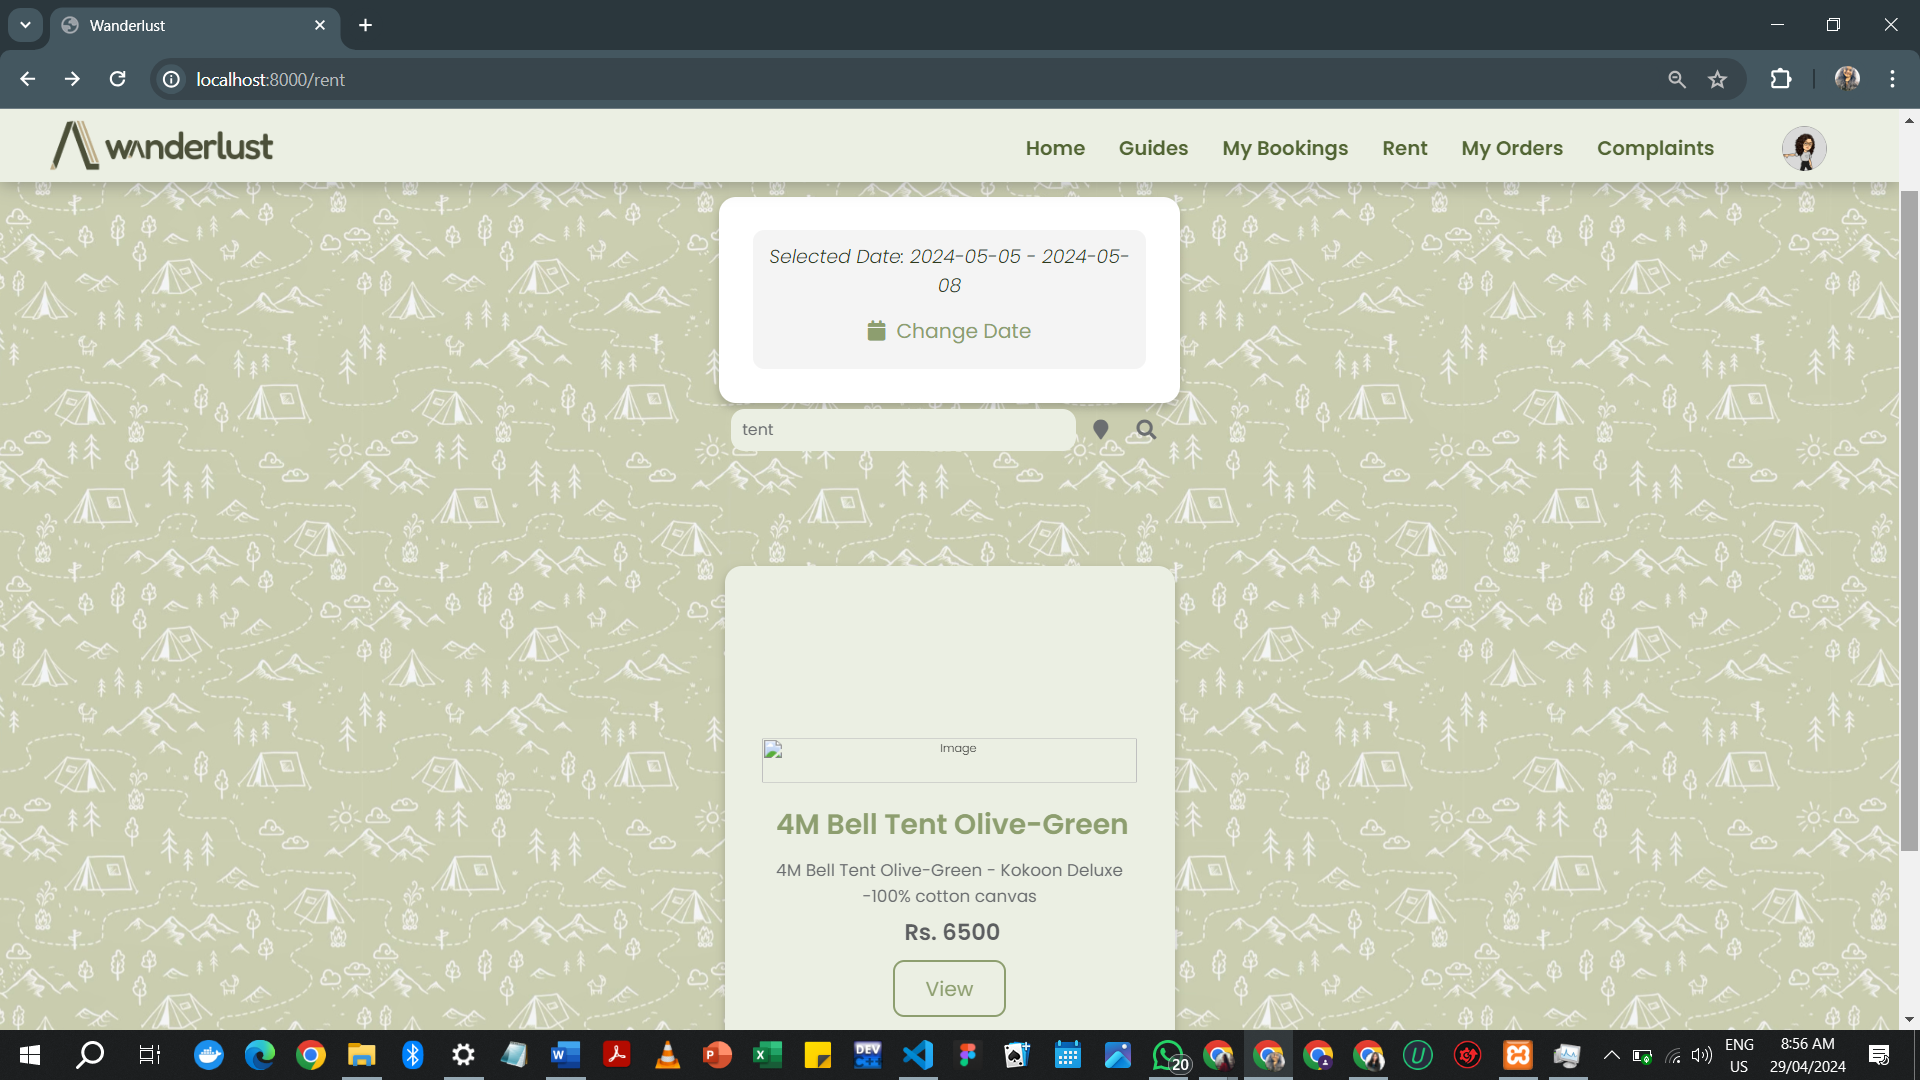
\includegraphics[width=1\textwidth]{Images/Test Cases/7. valid rent.png}
\end{figure}
\clearpage


\textbf{Booking and Buying Equipment}\\
\begin{table}[ht]
\centering
\begin{tabularx}{\textwidth}{|c|c|X|X|X|c|}
\hline
\textbf{TID} & \textbf{User Role} & \textbf{Scenario Description} & \textbf{Steps to Execute} & \textbf{Expected Result} & \textbf{Status} \\ \hline
8 & Customer & Adding the item to cart & 1.Select the item \newline2.Click add to cart & Item gets added to the cart & Pass \\ \hline
\end{tabularx}
\caption{Adding the item to cart}
\end{table}

\begin{figure}[h!]
    \centering
    \textbf{Actual Result}
    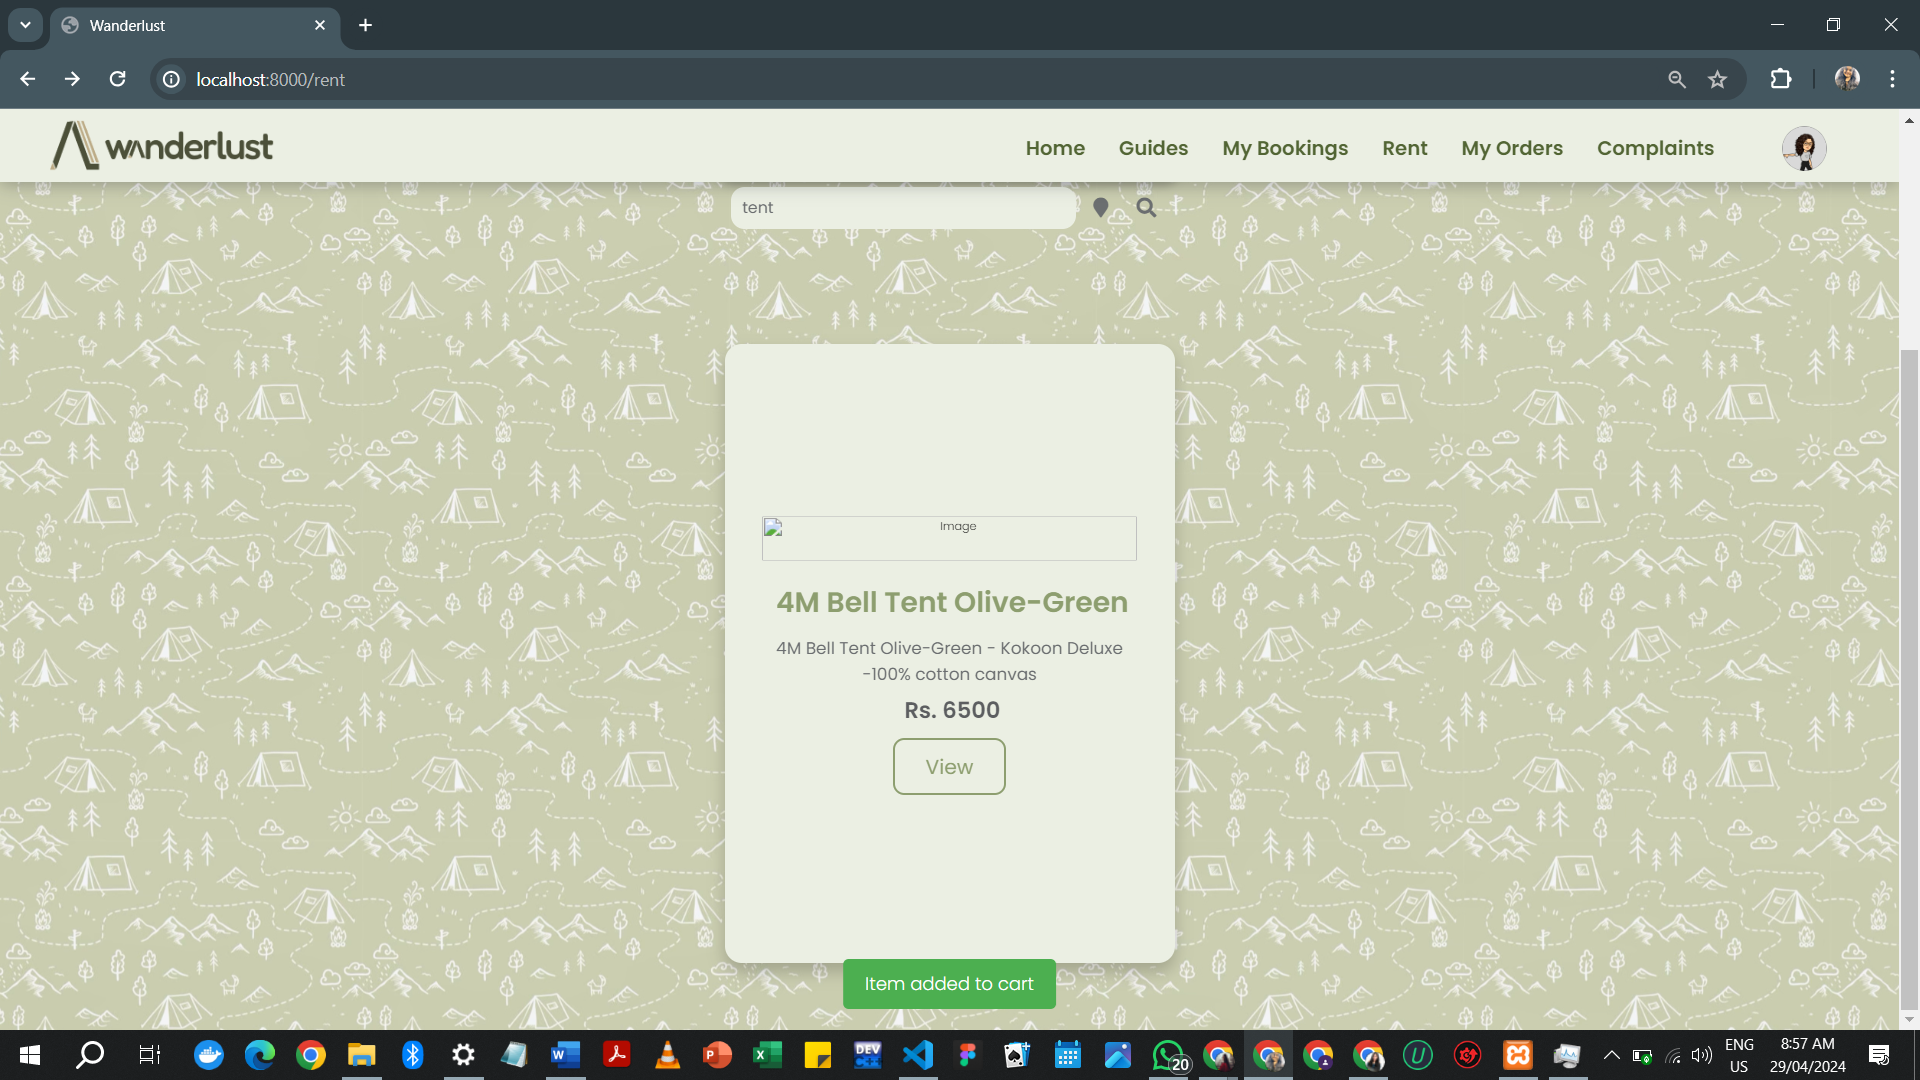
\includegraphics[width=1\textwidth]{Images/Test Cases/8. add to cart.png}
\end{figure}
\clearpage

\begin{table}[ht]
\centering
\begin{tabularx}{\textwidth}{|c|c|X|X|X|c|}
\hline
\textbf{TID} & \textbf{User Role} & \textbf{Scenario Description} & \textbf{Steps to Execute} & \textbf{Expected Result} & \textbf{Status} \\ \hline
9 & Customer & Buying equipment & 1.Select cart \newline2.Click payment method \newline3.Give necessary details \newline4.Click pay`& Payment is approved and order is pending & Pass \\ \hline
\end{tabularx}
\caption{Buying Equipment}
\end{table}

\begin{figure}[h!]
    \centering
    \textbf{Actual Result}
    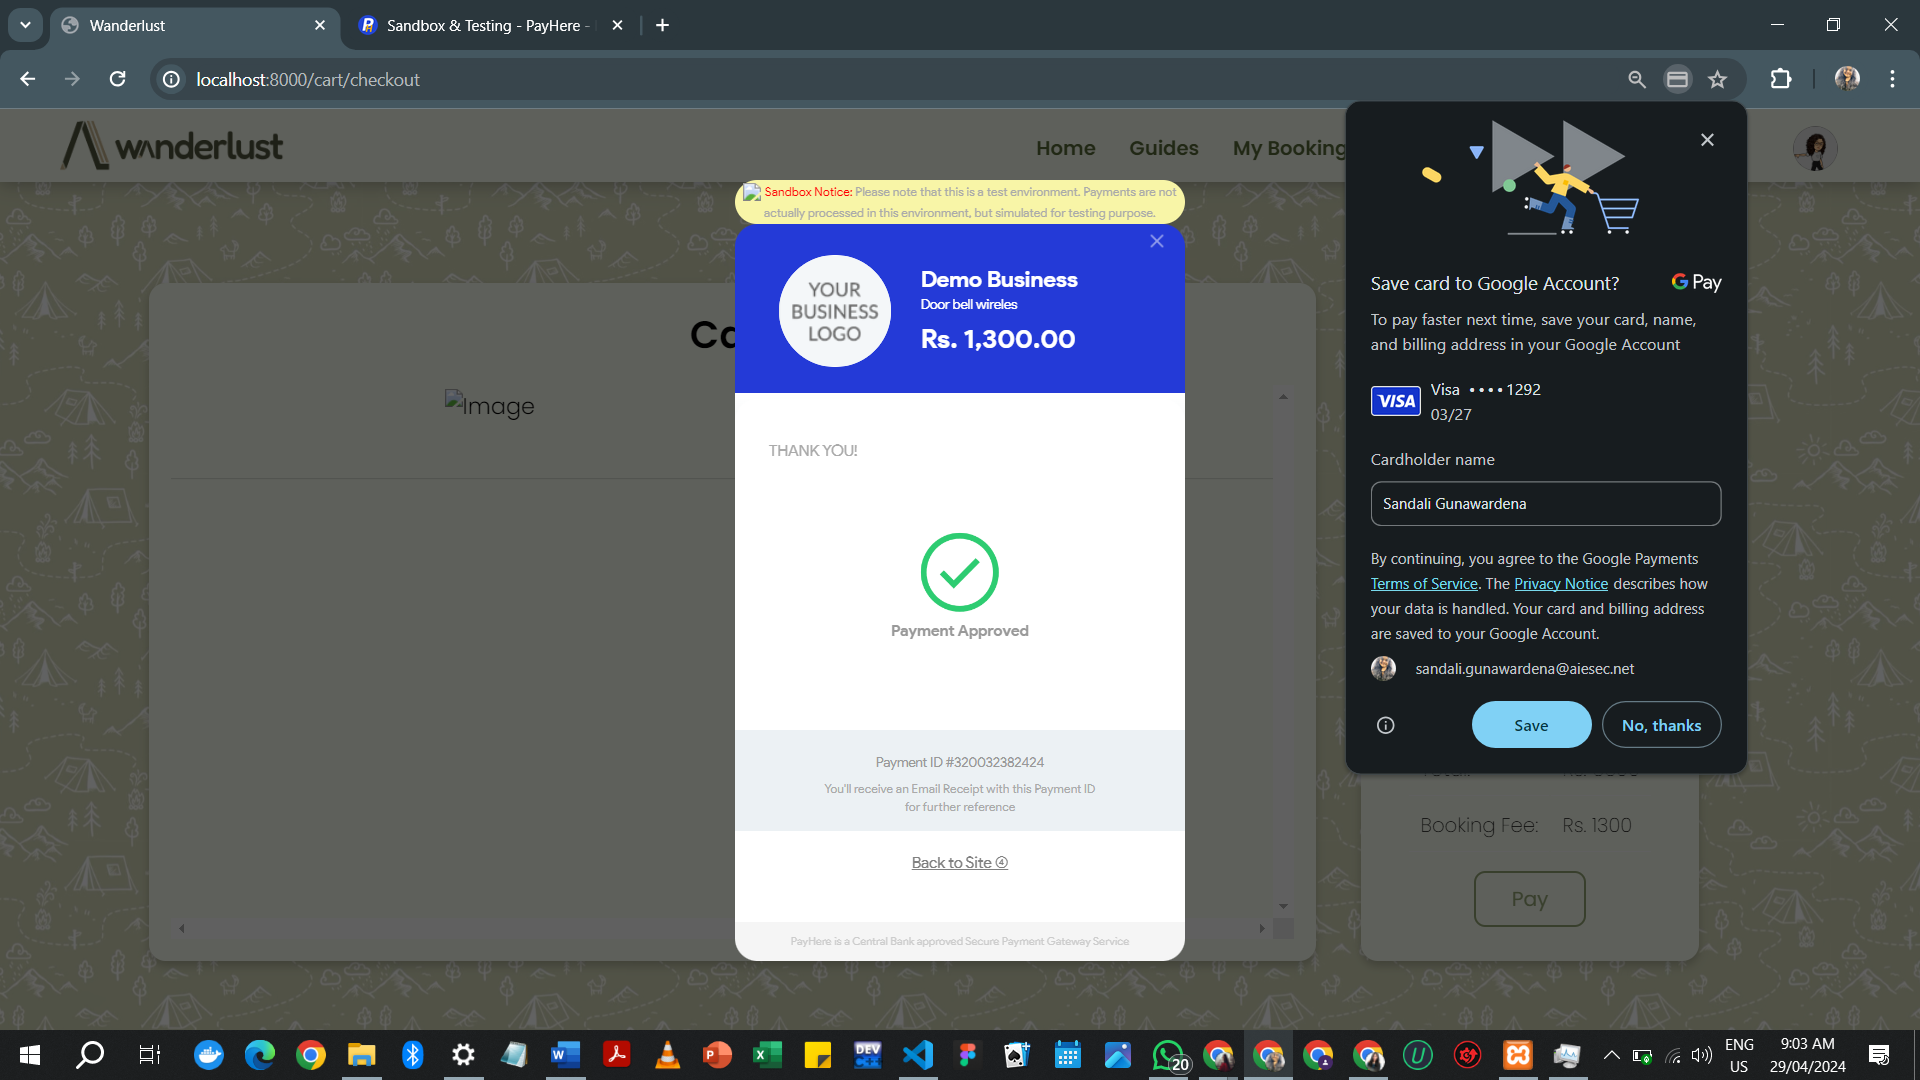
\includegraphics[width=1\textwidth]{Images/Test Cases/9. buy item.png}
\end{figure}
\clearpage

\textbf{Cancel orders}\\
\begin{table}[ht]
\centering
\begin{tabularx}{\textwidth}{|c|c|X|X|X|c|}
\hline
\textbf{TID} & \textbf{User Role} & \textbf{Scenario Description} & \textbf{Steps to Execute} & \textbf{Expected Result} & \textbf{Status} \\ \hline
10 & Customer & Cancelling order & 1.Select the order \newline2.Select cancel order \newline3.Confirm cancellation & Order gets cancelled & Pass \\ \hline
\end{tabularx}
\caption{Cancel orders}
\end{table}

\begin{figure}[h!]
    \centering
    \textbf{Actual Result}
    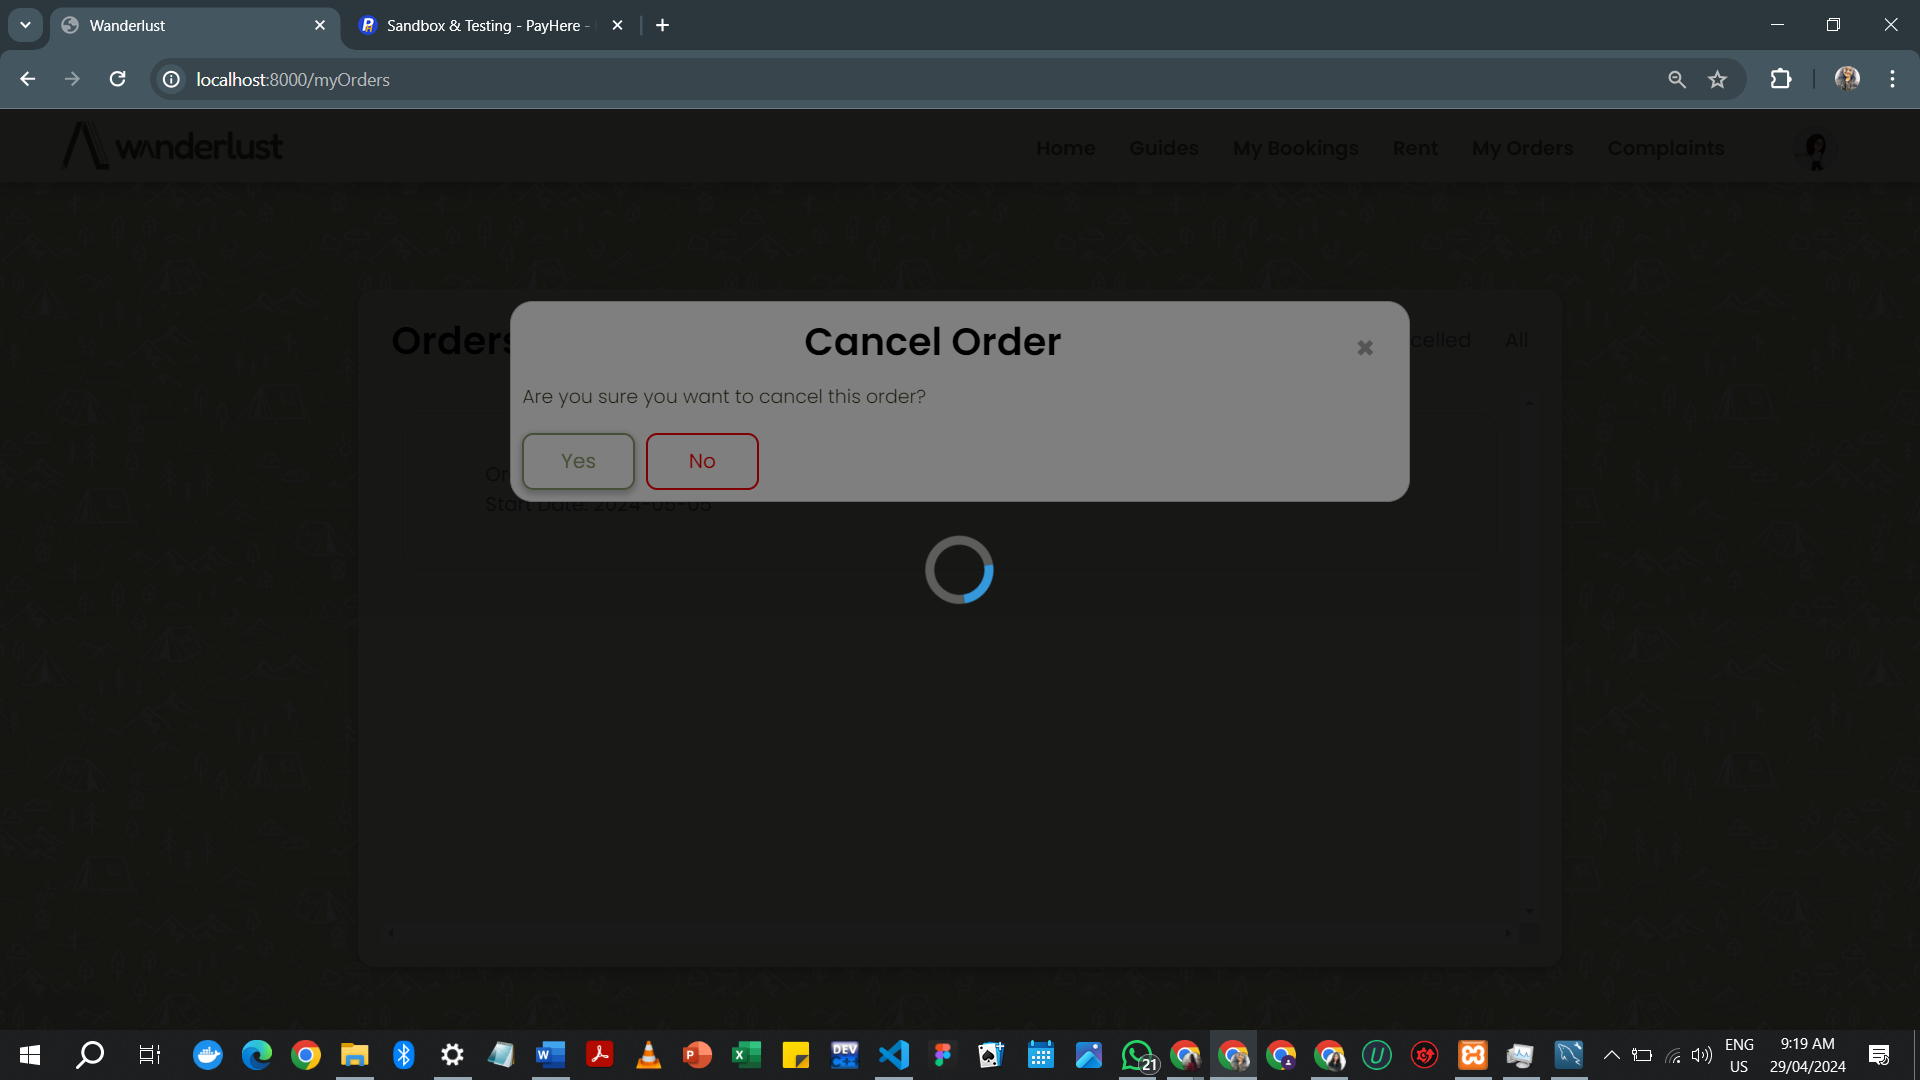
\includegraphics[width=1\textwidth]{Images/Test Cases/10. cancel order.png}
\end{figure}
\clearpage


\textbf{Search for guides}\\
\begin{table}[ht]
\centering
\begin{tabularx}{\textwidth}{|c|c|X|X|X|c|}
\hline
\textbf{TID} & \textbf{User Role} & \textbf{Scenario Description} & \textbf{Steps to Execute} & \textbf{Expected Result} & \textbf{Status} \\ \hline
11 & Customer & Searching for guides order & 1.Input date, location, and number of people \newline2.Click search & Available guides are displayed & Pass \\ \hline
\end{tabularx}
\caption{Search for guides}
\end{table}

\begin{figure}[h!]
    \centering
    \textbf{Actual Result}
    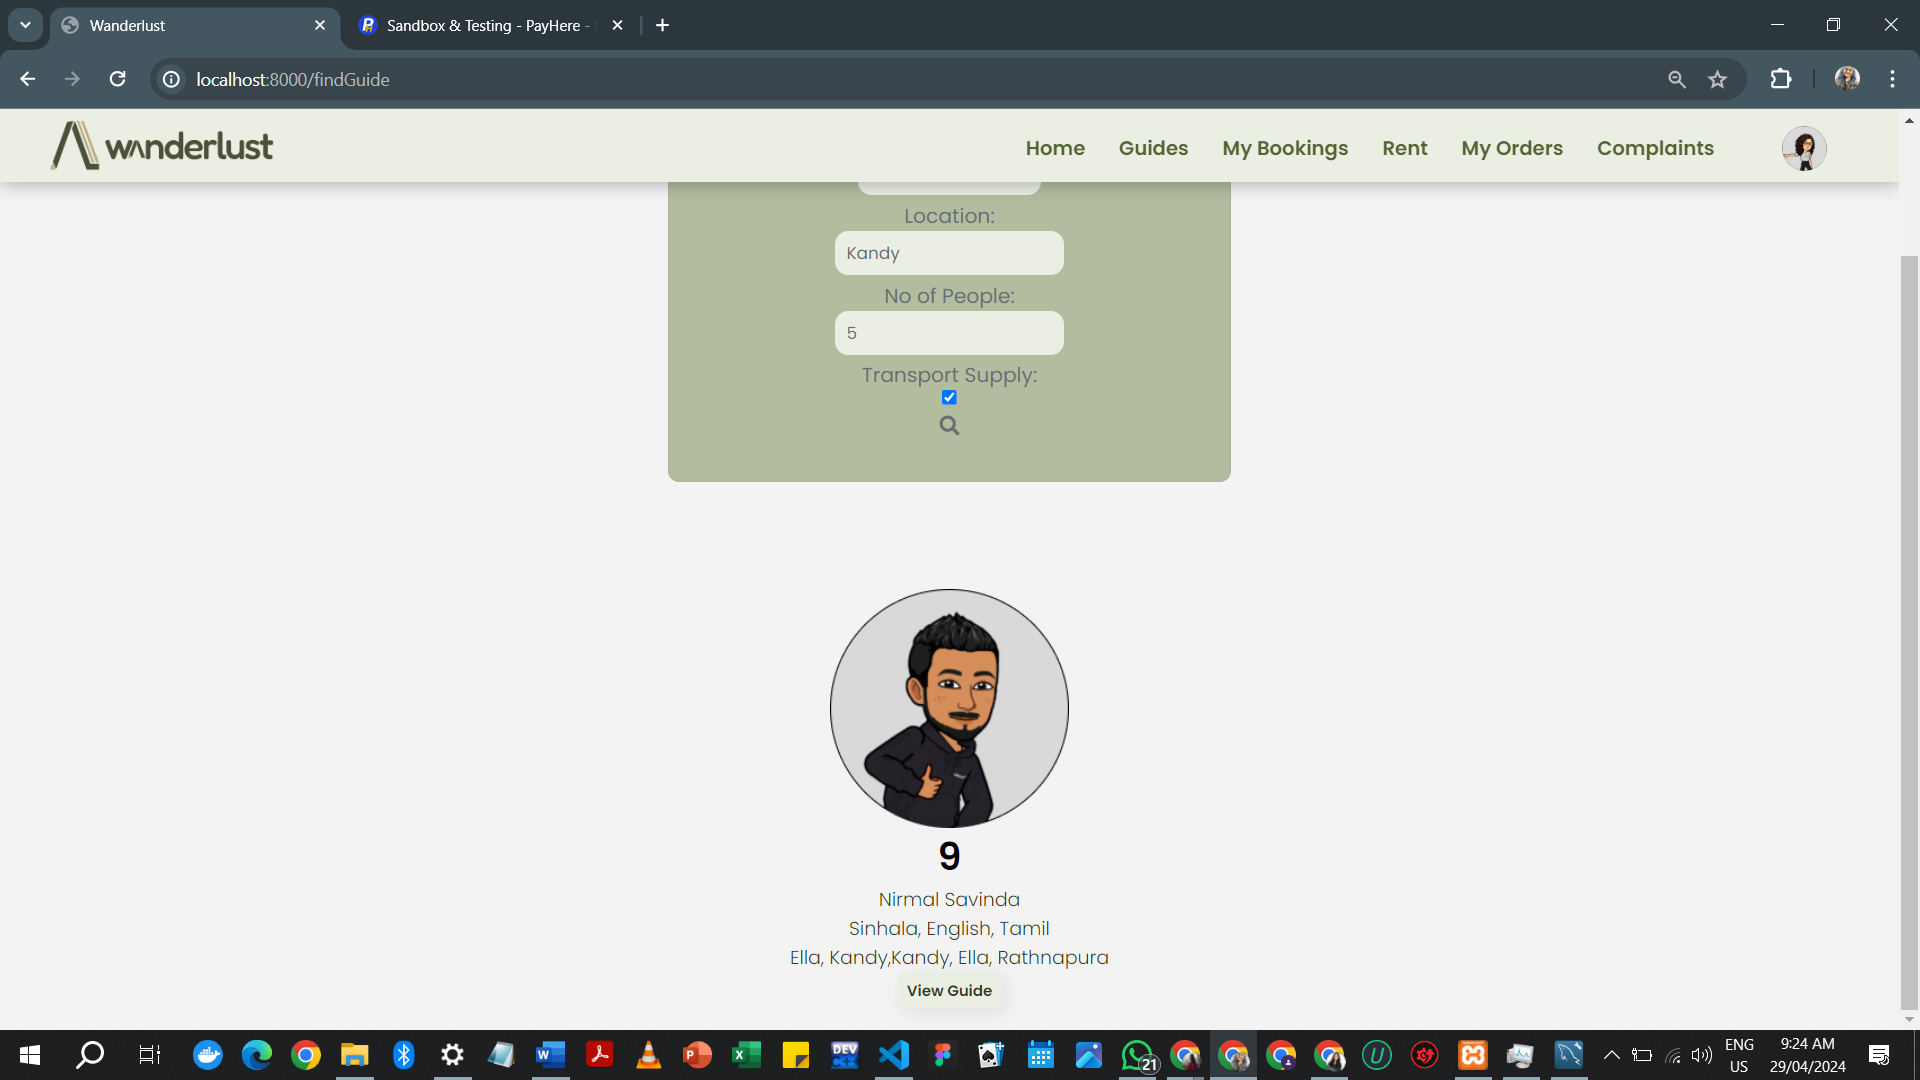
\includegraphics[width=1\textwidth]{Images/Test Cases/11. guide search.png}
\end{figure}
\clearpage


\textbf{Book guides}\\
\begin{table}[ht]
\centering
\begin{tabularx}{\textwidth}{|c|c|X|X|X|c|}
\hline
\textbf{TID} & \textbf{User Role} & \textbf{Scenario Description} & \textbf{Steps to Execute} & \textbf{Expected Result} & \textbf{Status} \\ \hline
12 & Customer & Booking guides & 1.Select the guide and the required package \newline2.Click book \newline3.Confirm payment \newline4.Fill the necessary payment details \newline5.Make payment & Guide is booked & Pass \\ \hline
\end{tabularx}
\caption{Book guides}
\end{table}

\begin{figure}[h!]
    \centering
    \textbf{Actual Result}
    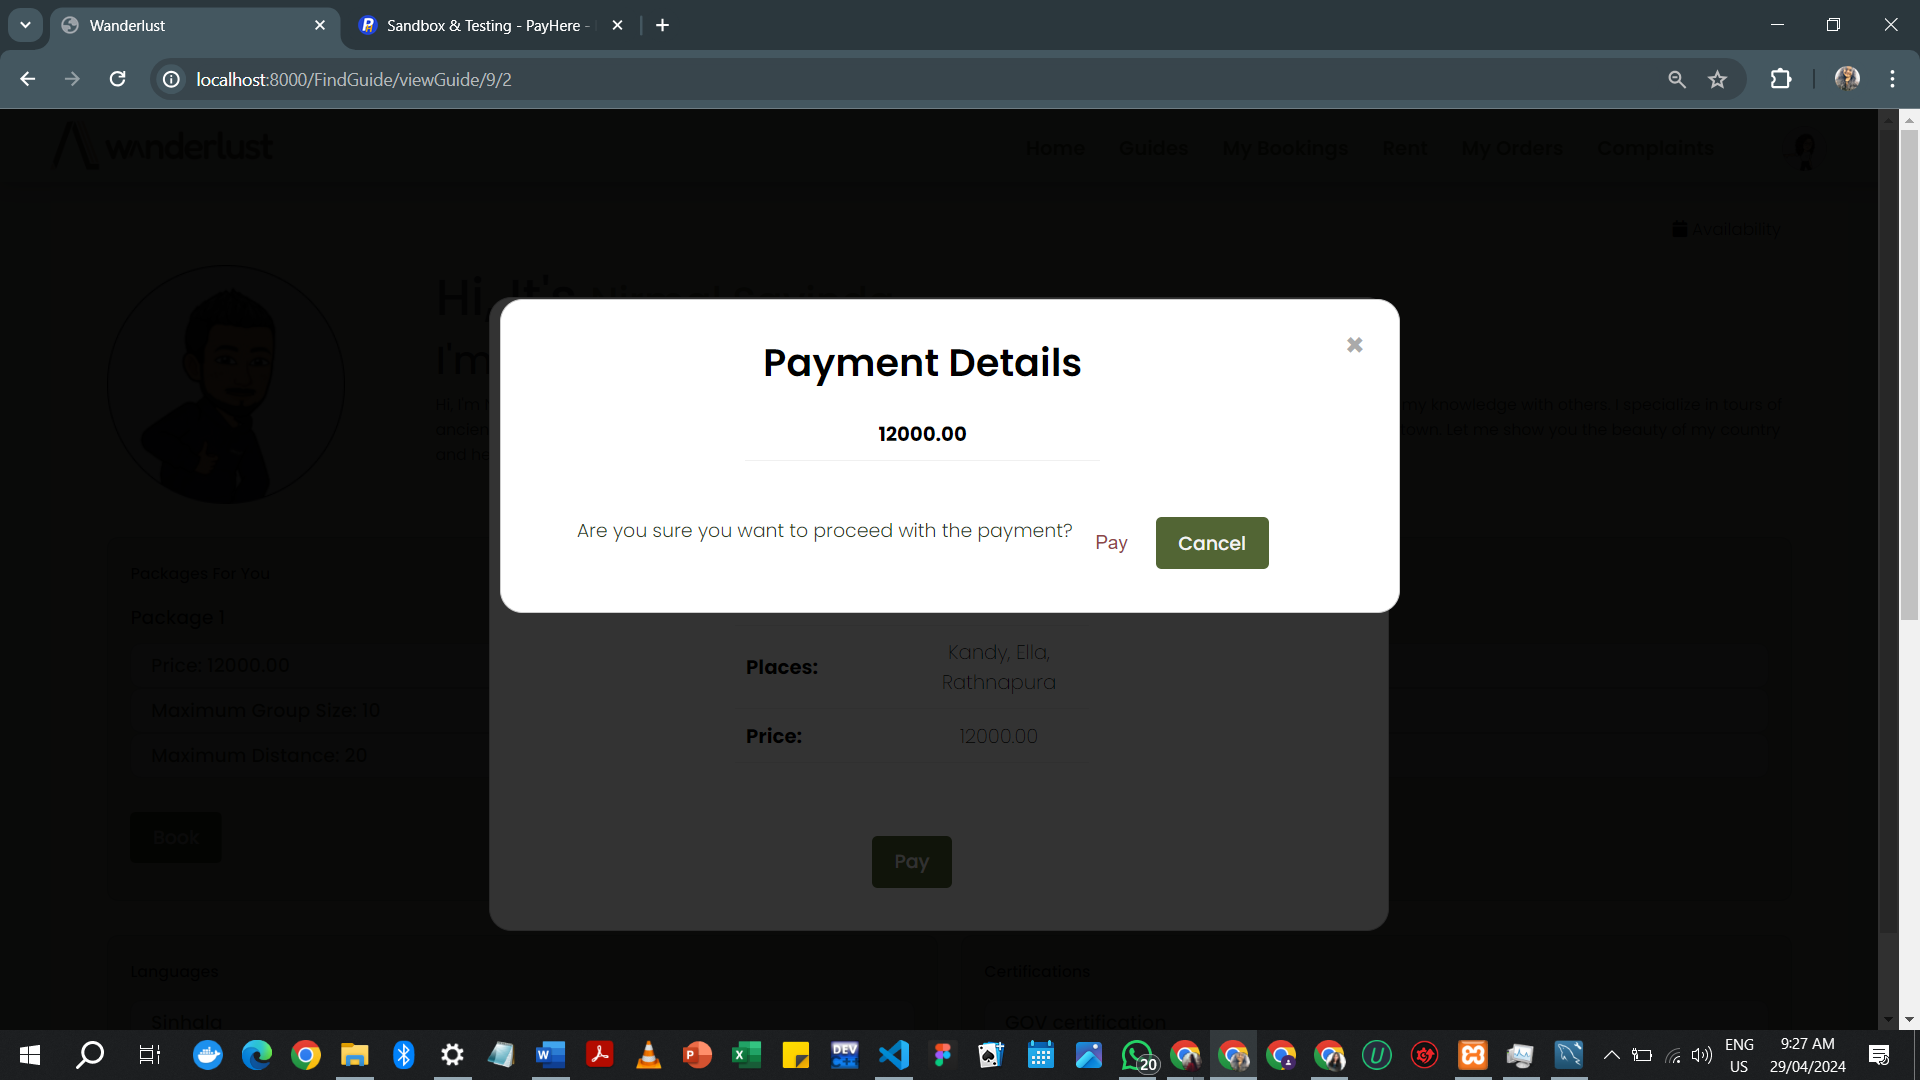
\includegraphics[width=1\textwidth]{Images/Test Cases/12. book guide.png}
\end{figure}
\clearpage


\textbf{Make complaints}\\
\begin{table}[ht]
\centering
\begin{tabularx}{\textwidth}{|c|c|X|X|X|c|}
\hline
\textbf{TID} & \textbf{User Role} & \textbf{Scenario Description} & \textbf{Steps to Execute} & \textbf{Expected Result} & \textbf{Status} \\ \hline
13 & Customer & Making complaints of rented items & 1.Select My Orders \newline2.Go to upcoming tab \newline3.Click complain if the required item \newline4.Make the complaint & Complaint is in "Complains" page & Pass \\ \hline
\end{tabularx}
\caption{Make complaints}
\end{table}

\begin{figure}[h!]
    \centering
    \textbf{Actual Result}
    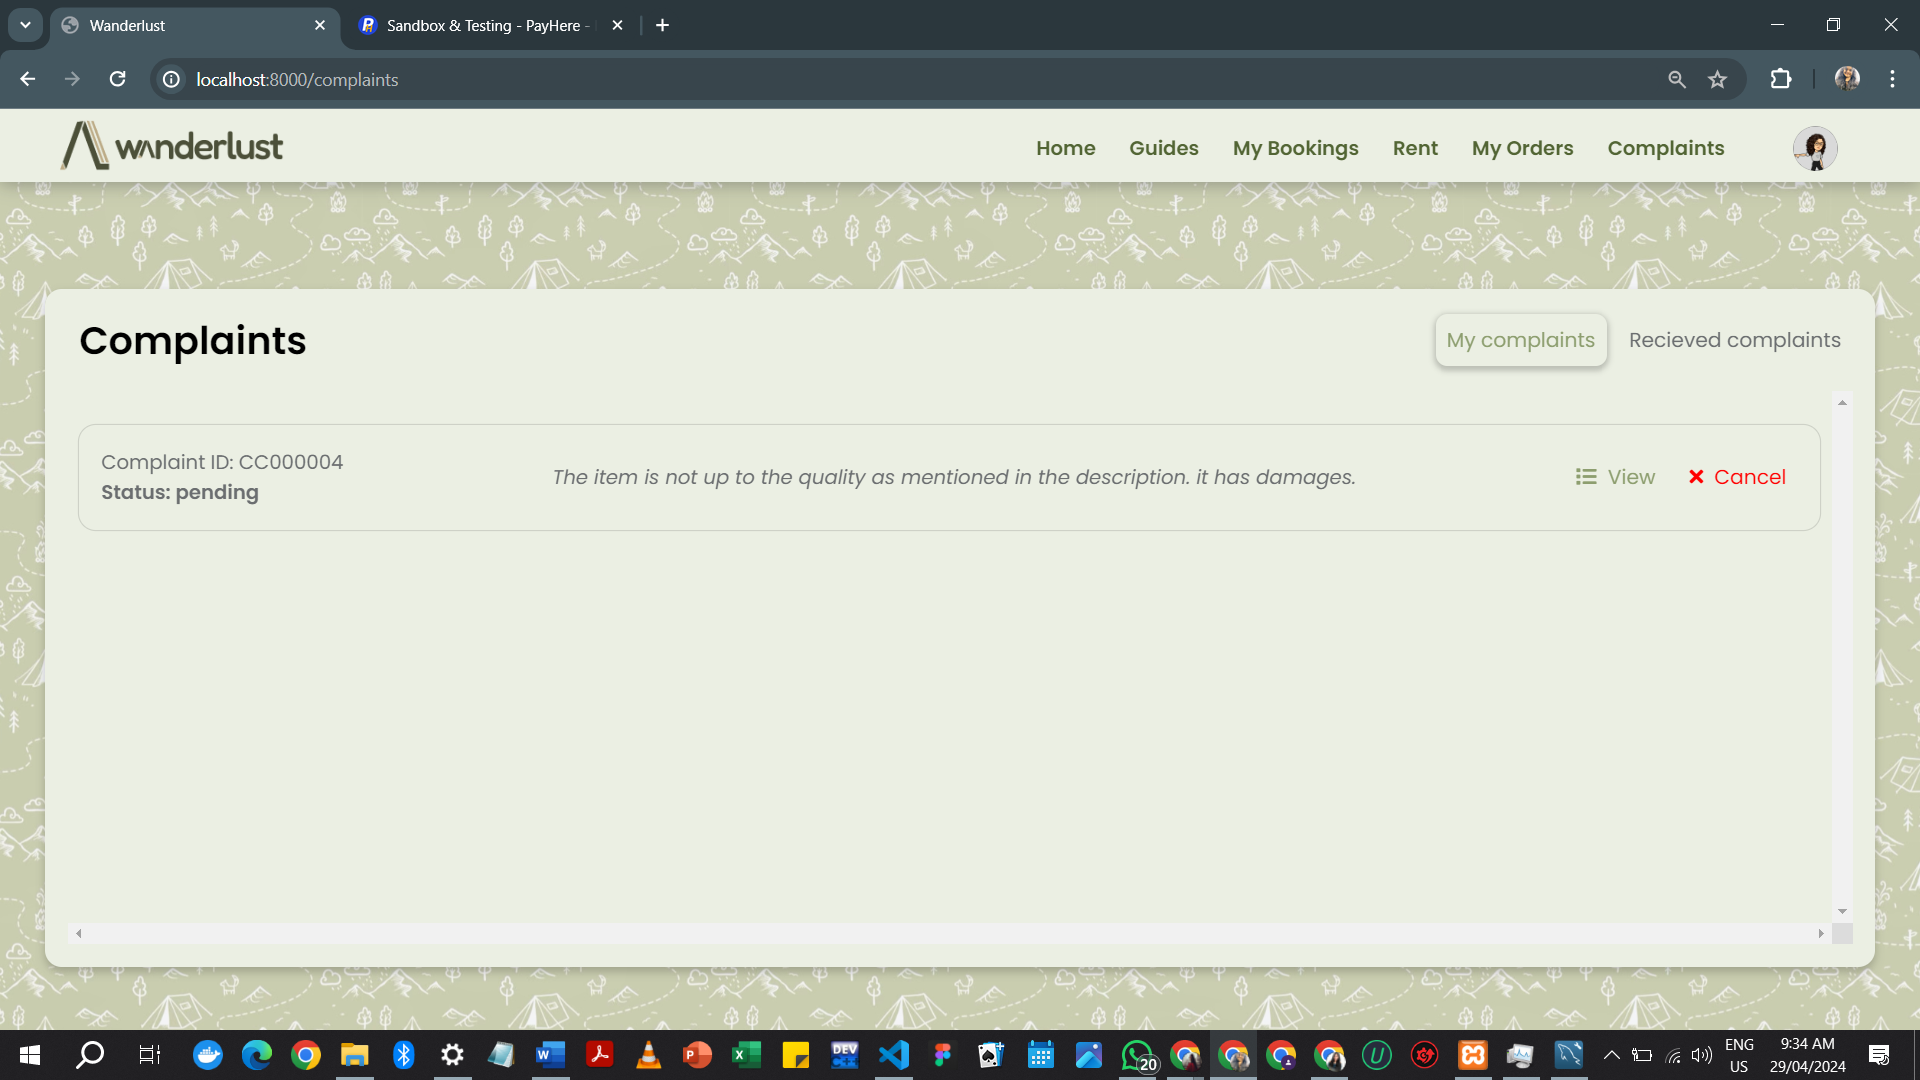
\includegraphics[width=1\textwidth]{Images/Test Cases/13. make complaints.png}
\end{figure}
\clearpage


\textbf{Guide Profile Editing}\\
\begin{table}[ht]
\centering
\begin{tabularx}{\textwidth}{|c|c|X|X|X|c|}
\hline
\textbf{TID} & \textbf{User Role} & \textbf{Scenario Description} & \textbf{Steps to Execute} & \textbf{Expected Result} & \textbf{Status} \\ \hline
14 & Guide & Profile editing & 1.Select 'Edit Profile' \newline2.Enter the new details \newline3.Click Update & Profile is updated & Pass \\ \hline
\end{tabularx}
\caption{Edit profile}
\end{table}

\begin{figure}[h!]
    \centering
    \textbf{Actual Result}
    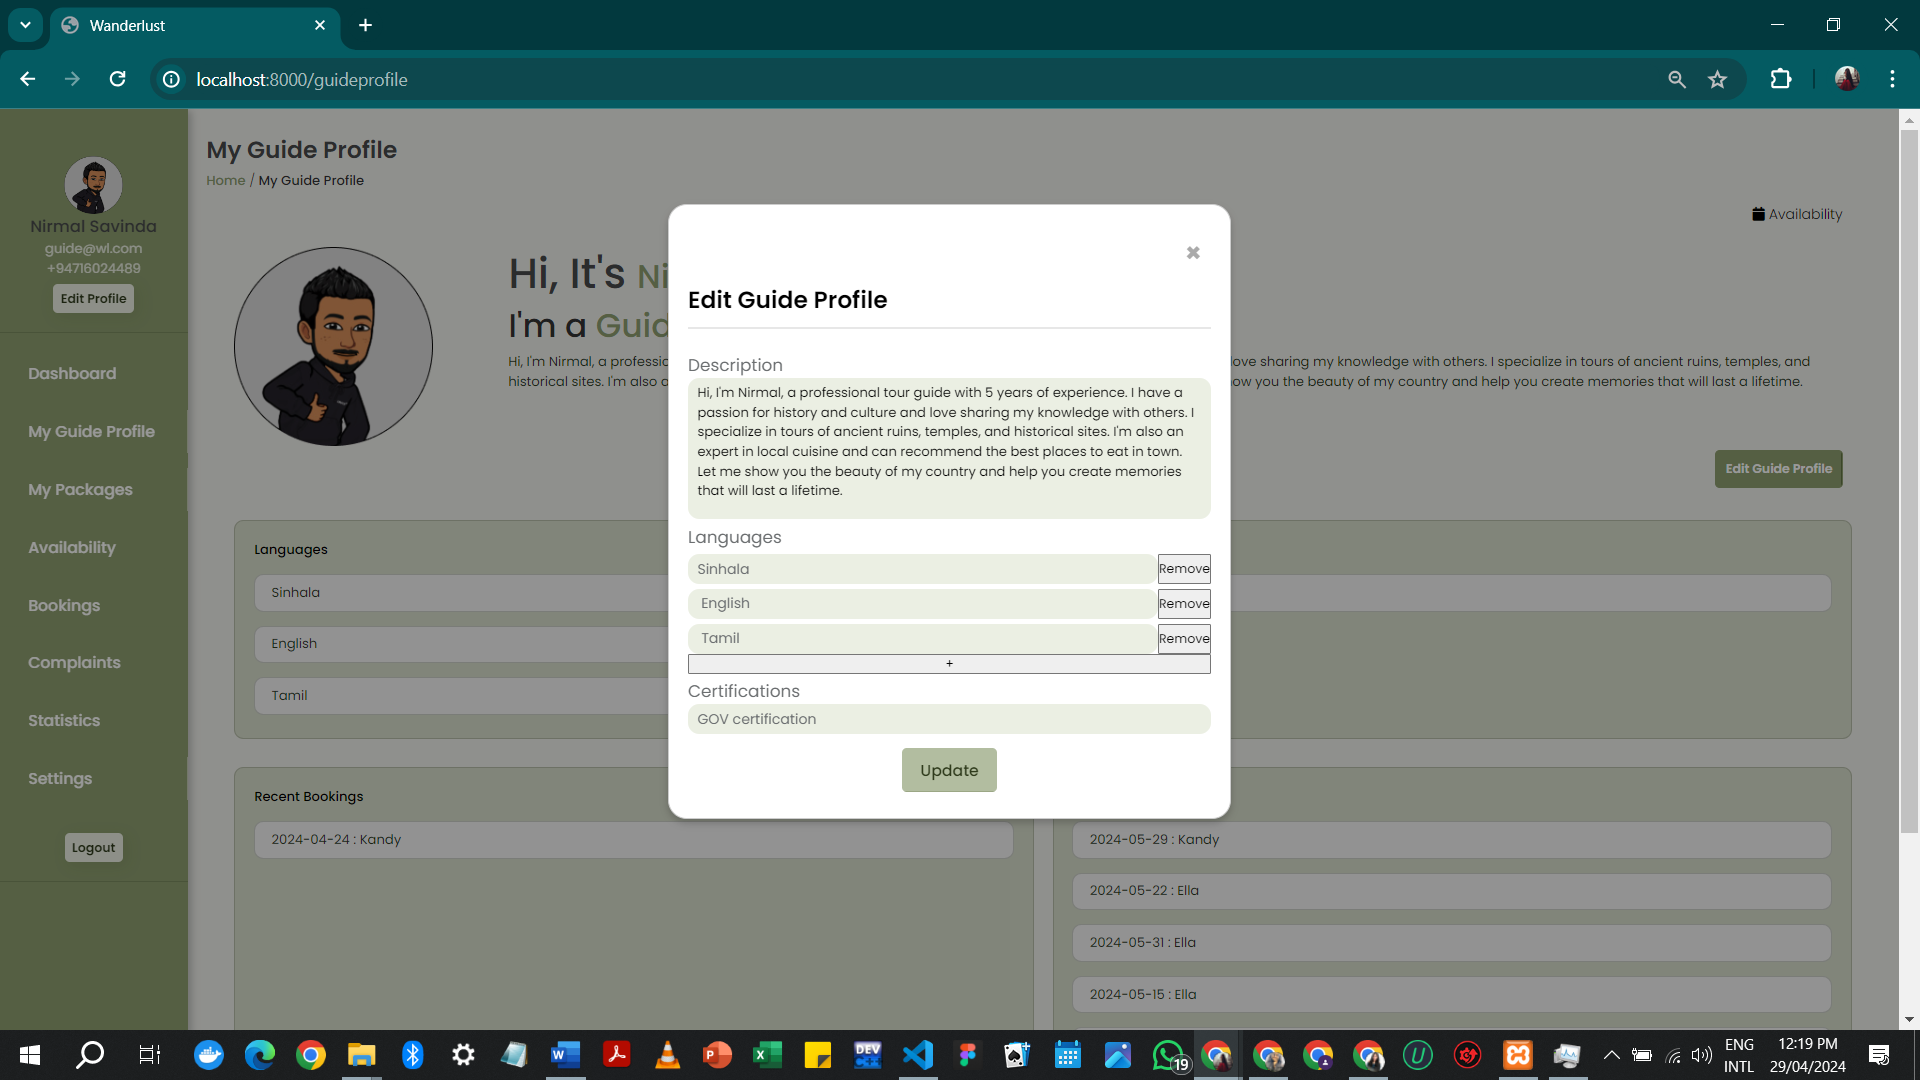
\includegraphics[width=1\textwidth]{Images/Test Cases/14. profile edit.png}
\end{figure}
\clearpage


\textbf{Updating Calendar Availability}\\
\begin{table}[ht]
\centering
\begin{tabularx}{\textwidth}{|c|c|X|X|X|c|}
\hline
\textbf{TID} & \textbf{User Role} & \textbf{Scenario Description} & \textbf{Steps to Execute} & \textbf{Expected Result} & \textbf{Status} \\ \hline
15 & Guide & Invalid calendar availability update & 1.Select an old date to update the calendar availability & Calendar is not responding & Pass \\ \hline
\end{tabularx}
\caption{Invalid calendar availability update}
\end{table}

\begin{figure}[h!]
    \centering
    \textbf{Actual Result}
    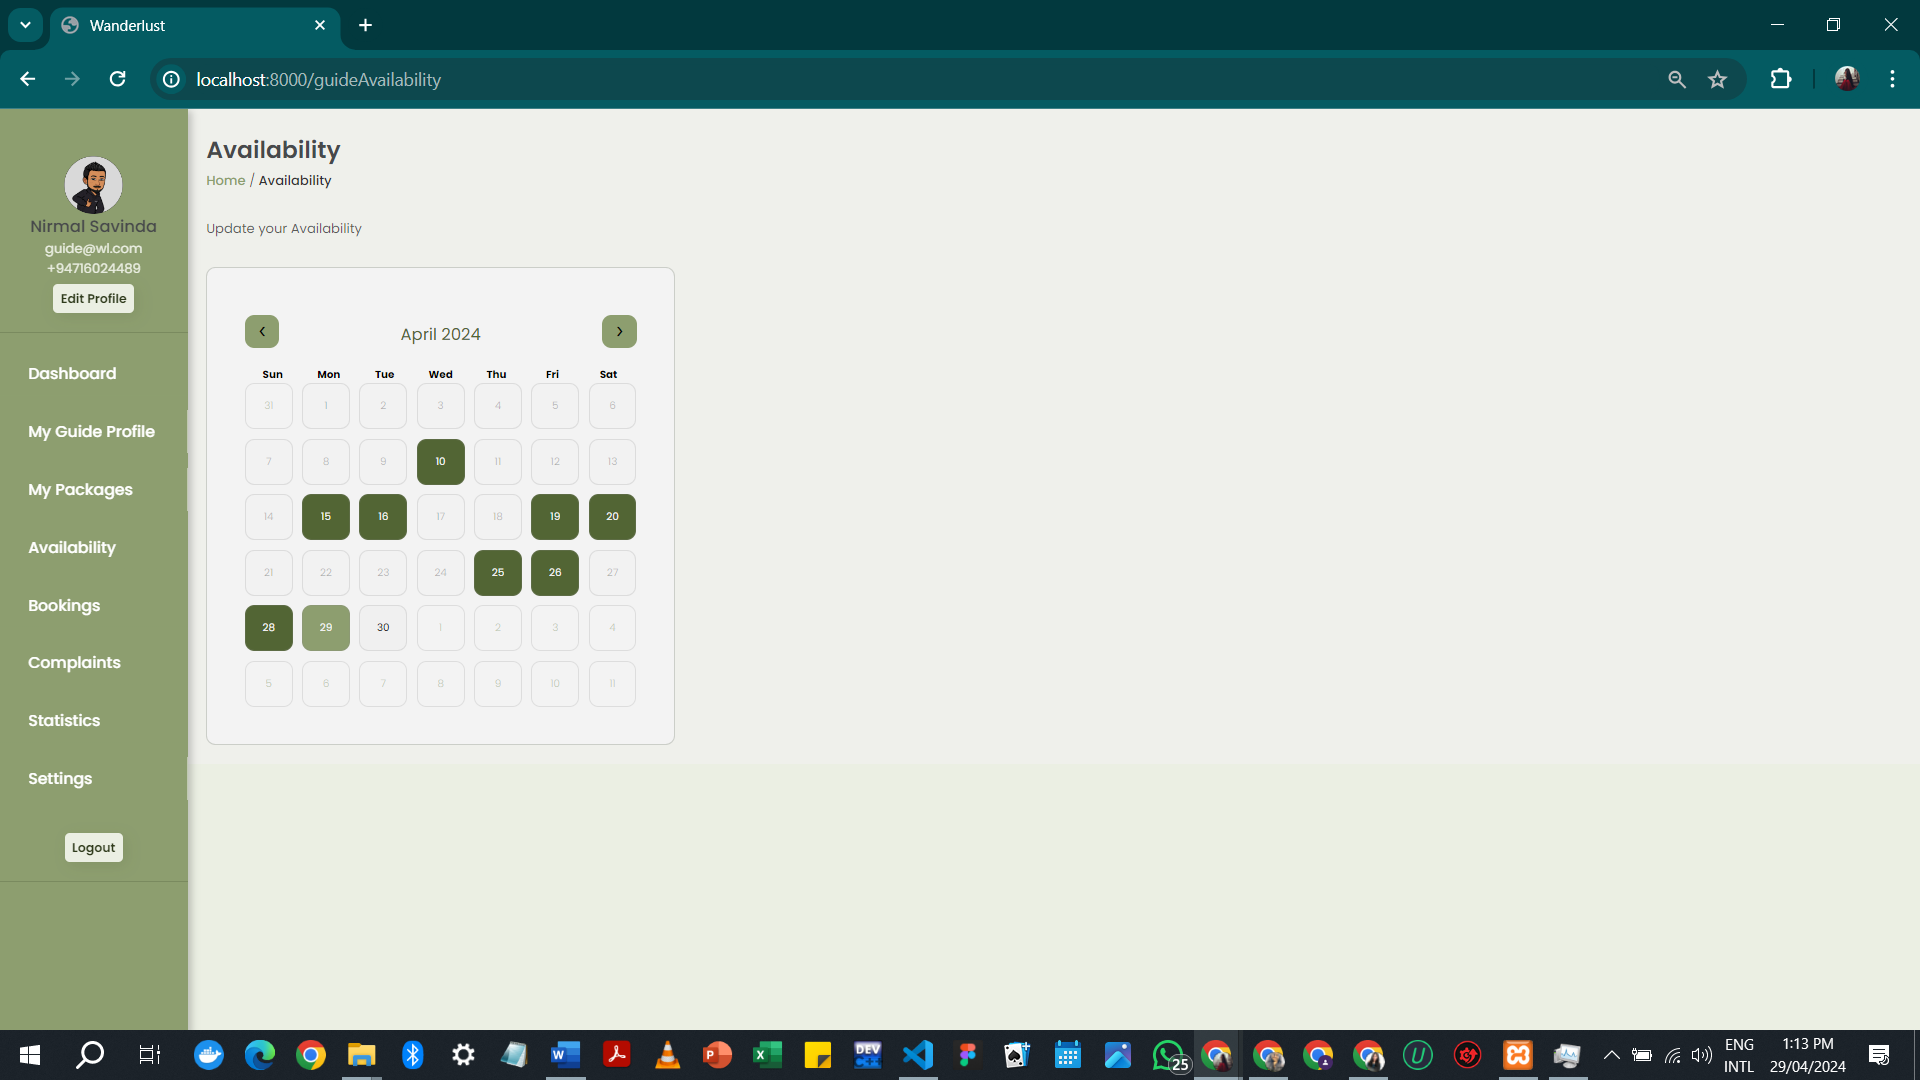
\includegraphics[width=1\textwidth]{Images/Test Cases/15. invalid Calendar availability.png}
\end{figure}
\clearpage



\begin{table}[ht]
\centering
\begin{tabularx}{\textwidth}{|c|c|X|X|X|c|}
\hline
\textbf{TID} & \textbf{User Role} & \textbf{Scenario Description} & \textbf{Steps to Execute} & \textbf{Expected Result} & \textbf{Status} \\ \hline
16 & Guide & Valid calendar availability update & 1.Select a valid date to update \newline2.Click Update & Calendar availability 
 is updated & Pass \\ \hline
\end{tabularx}
\caption{Valid calendar availability update}
\end{table}

\begin{figure}[h!]
    \centering
    \textbf{Actual Result}
    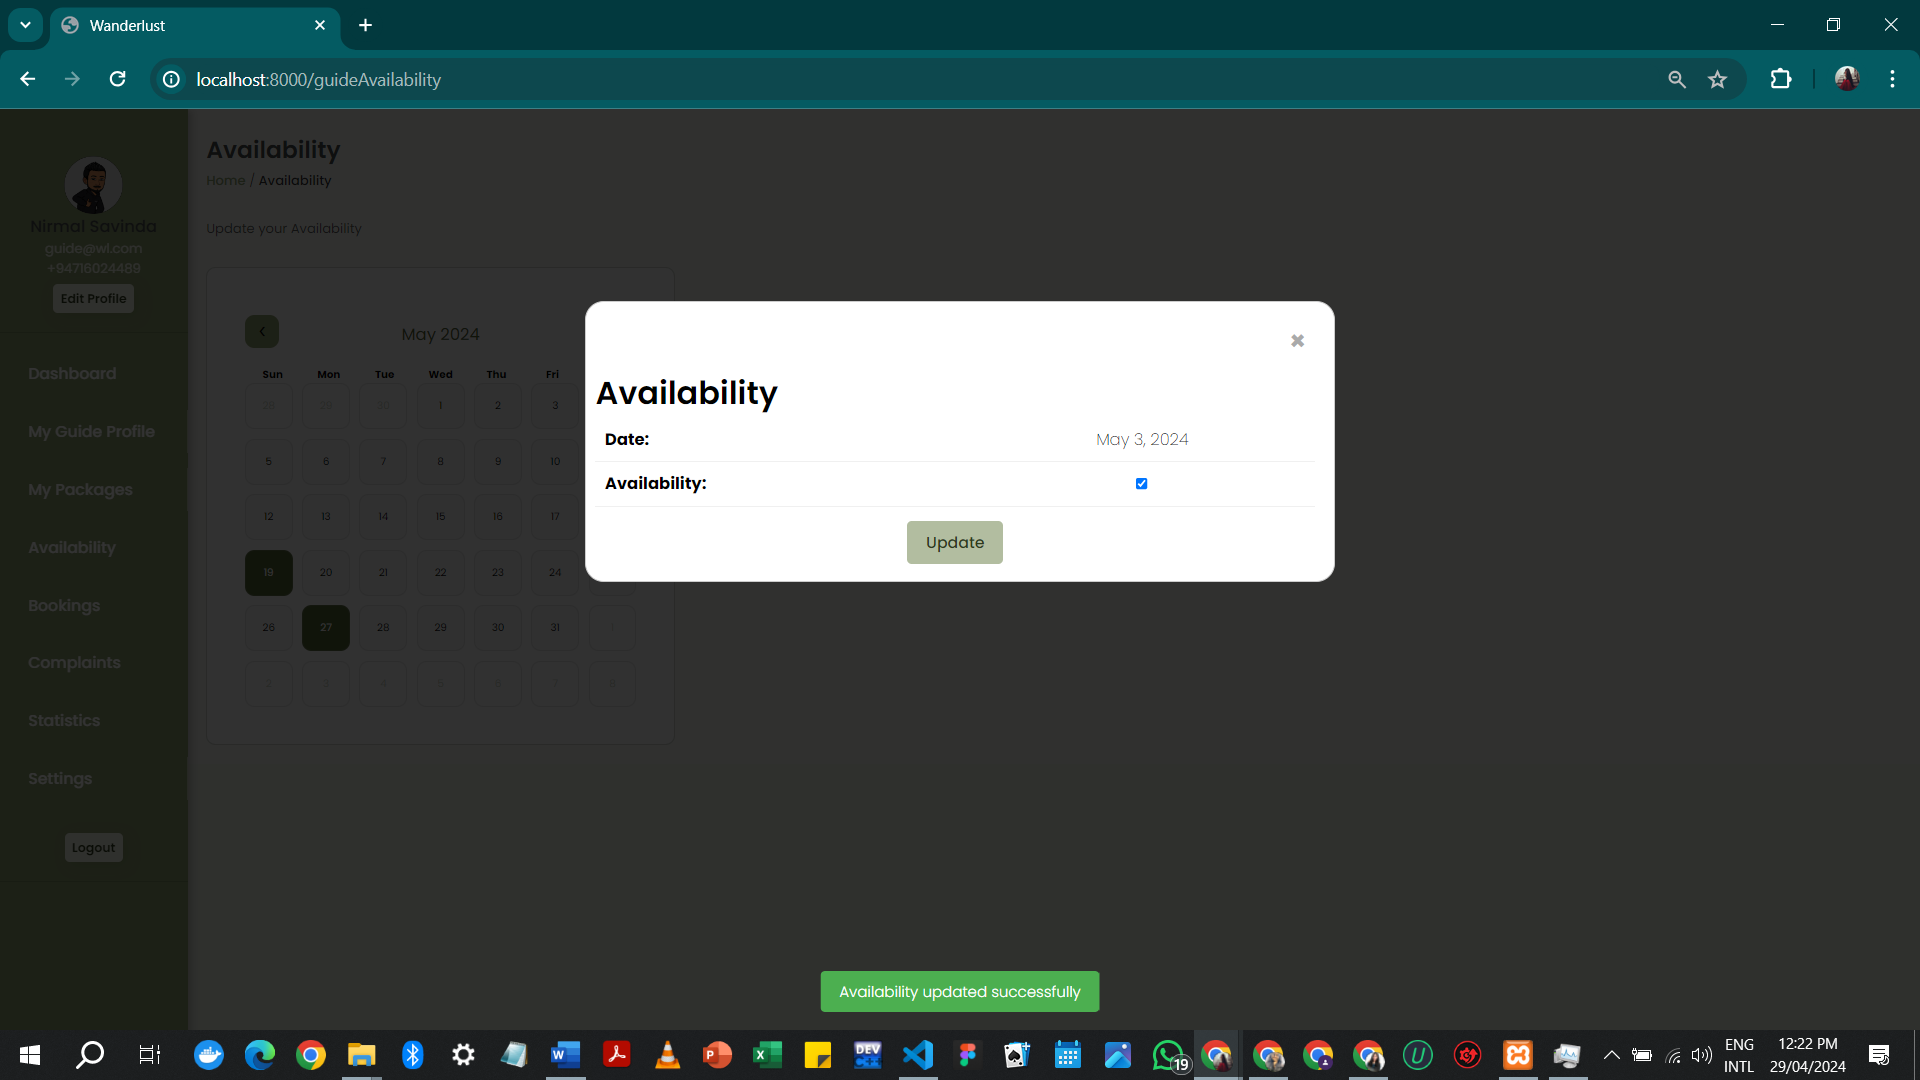
\includegraphics[width=1\textwidth]{Images/Test Cases/16. change calendar availability.png}
\end{figure}
\clearpage


% \textbf{Guide Package}\\
% \begin{table}[ht]
% \centering
% \begin{tabularx}{\textwidth}{|c|c|X|X|X|c|}
% \hline
% \textbf{TID} & \textbf{User Role} & \textbf{Scenario Description} & \textbf{Steps to Execute} & \textbf{Expected Result} & \textbf{Status} \\ \hline
% 17 & Guide & Guide Package updating & 1.Selecting an invalid time range for the input \newline2. Click Generate Report & Error message pops up & Pass \\ \hline
% \end{tabularx}
% \caption{Invalid data given for the report}
% \end{table}

% \begin{figure}[h!]
%     \centering
%     \textbf{Actual Result}
%     % \includegraphics[width=1\textwidth]{Images/Test Cases/}
% \end{figure}
% \clearpage


\textbf{Report Generation}\\
\begin{table}[ht]
\centering
\begin{tabularx}{\textwidth}{|c|c|X|X|X|c|}
\hline
\textbf{TID} & \textbf{User Role} & \textbf{Scenario Description} & \textbf{Steps to Execute} & \textbf{Expected Result} & \textbf{Status} \\ \hline
18 & Guide & Invalid Report generation & 1.Selecting an invalid time range for the input \newline2. Click Generate Report & Error message pops up & Pass \\ \hline
\end{tabularx}
\caption{Invalid data given for the report}
\end{table}

\begin{figure}[h!]
    \centering
    \textbf{Actual Result}
    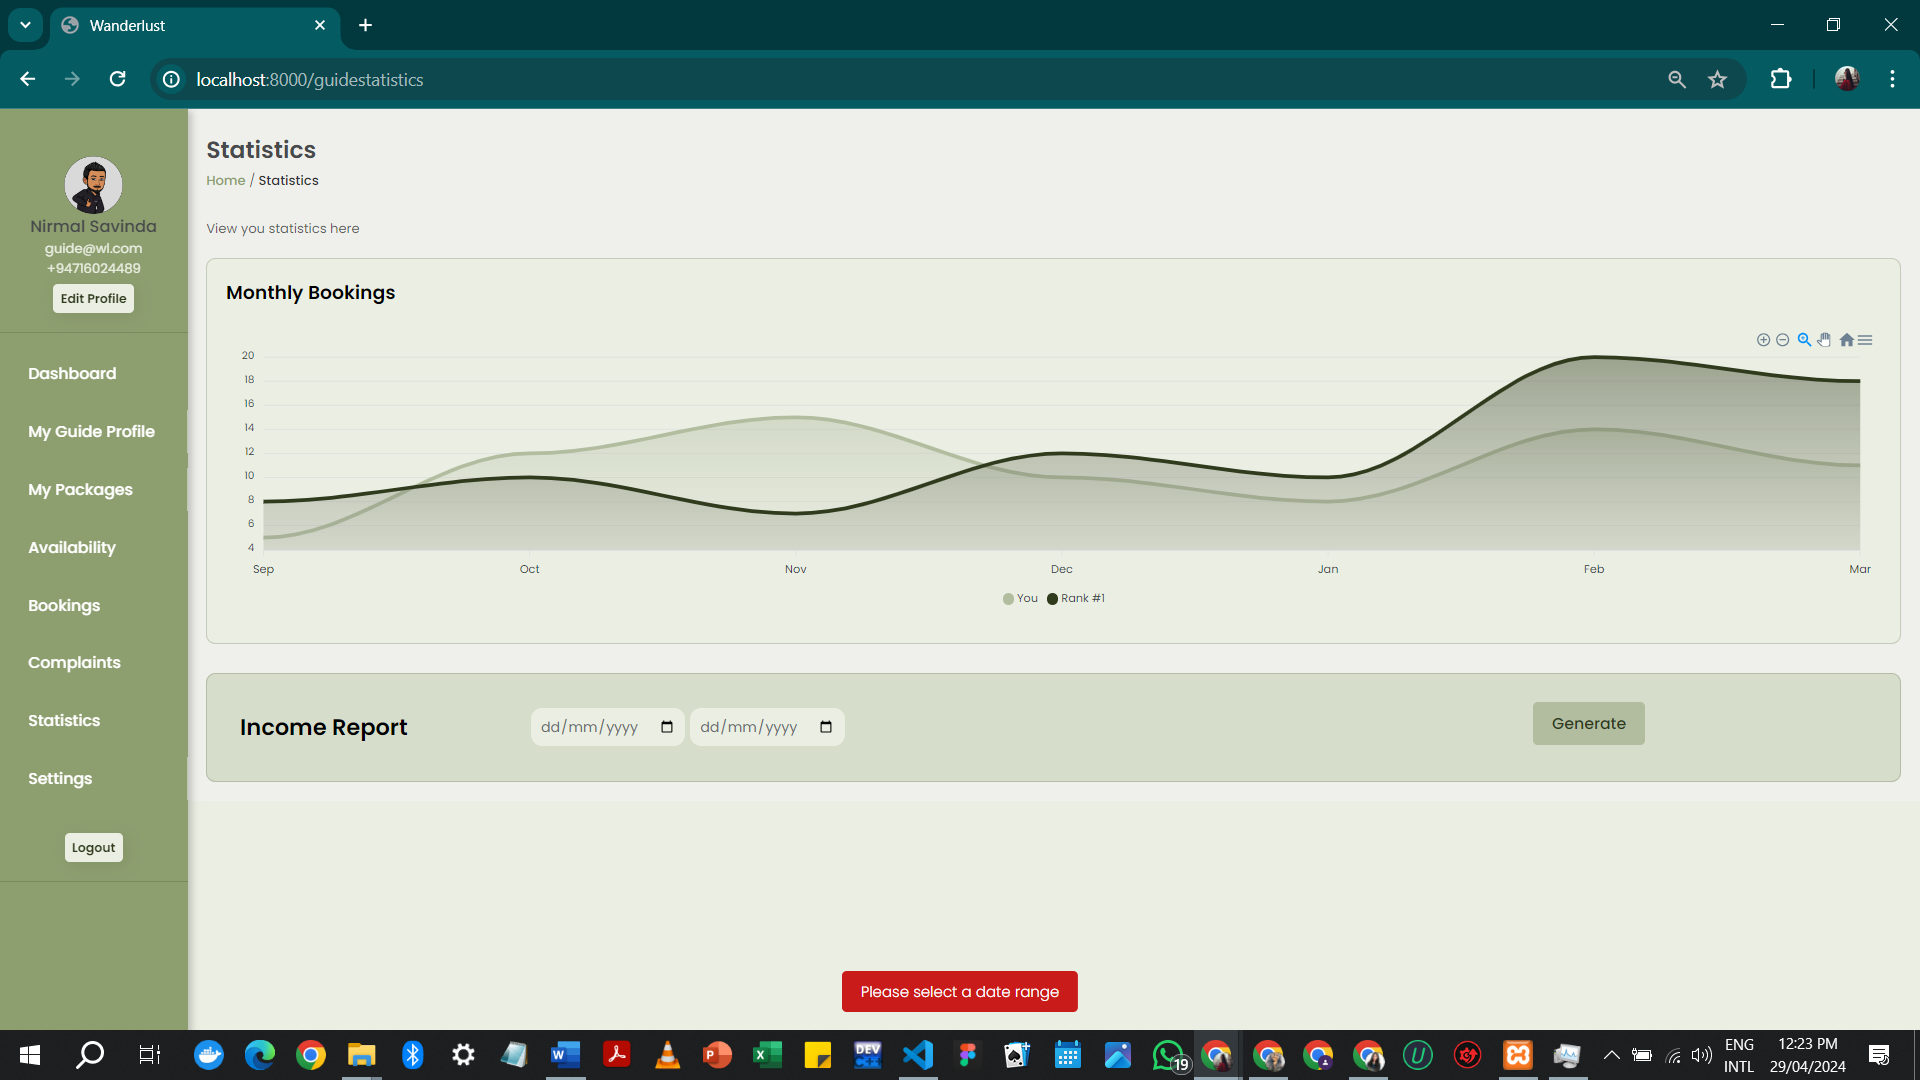
\includegraphics[width=1\textwidth]{Images/Test Cases/18. invalid report.png}
\end{figure}
\clearpage


\begin{table}[ht]
\centering
\begin{tabularx}{\textwidth}{|c|c|X|X|X|c|}
\hline
\textbf{TID} & \textbf{User Role} & \textbf{Scenario Description} & \textbf{Steps to Execute} & \textbf{Expected Result} & \textbf{Status} \\ \hline
19 & Guide & Valid Report generation & 1.Selecting a valid time range for the input \newline2. Click Generate Report & Report is generated & Pass \\ \hline
\end{tabularx}
\caption{Valid data given for the report}
\end{table}

\begin{figure}[h!]
    \centering
    \textbf{Actual Result}
    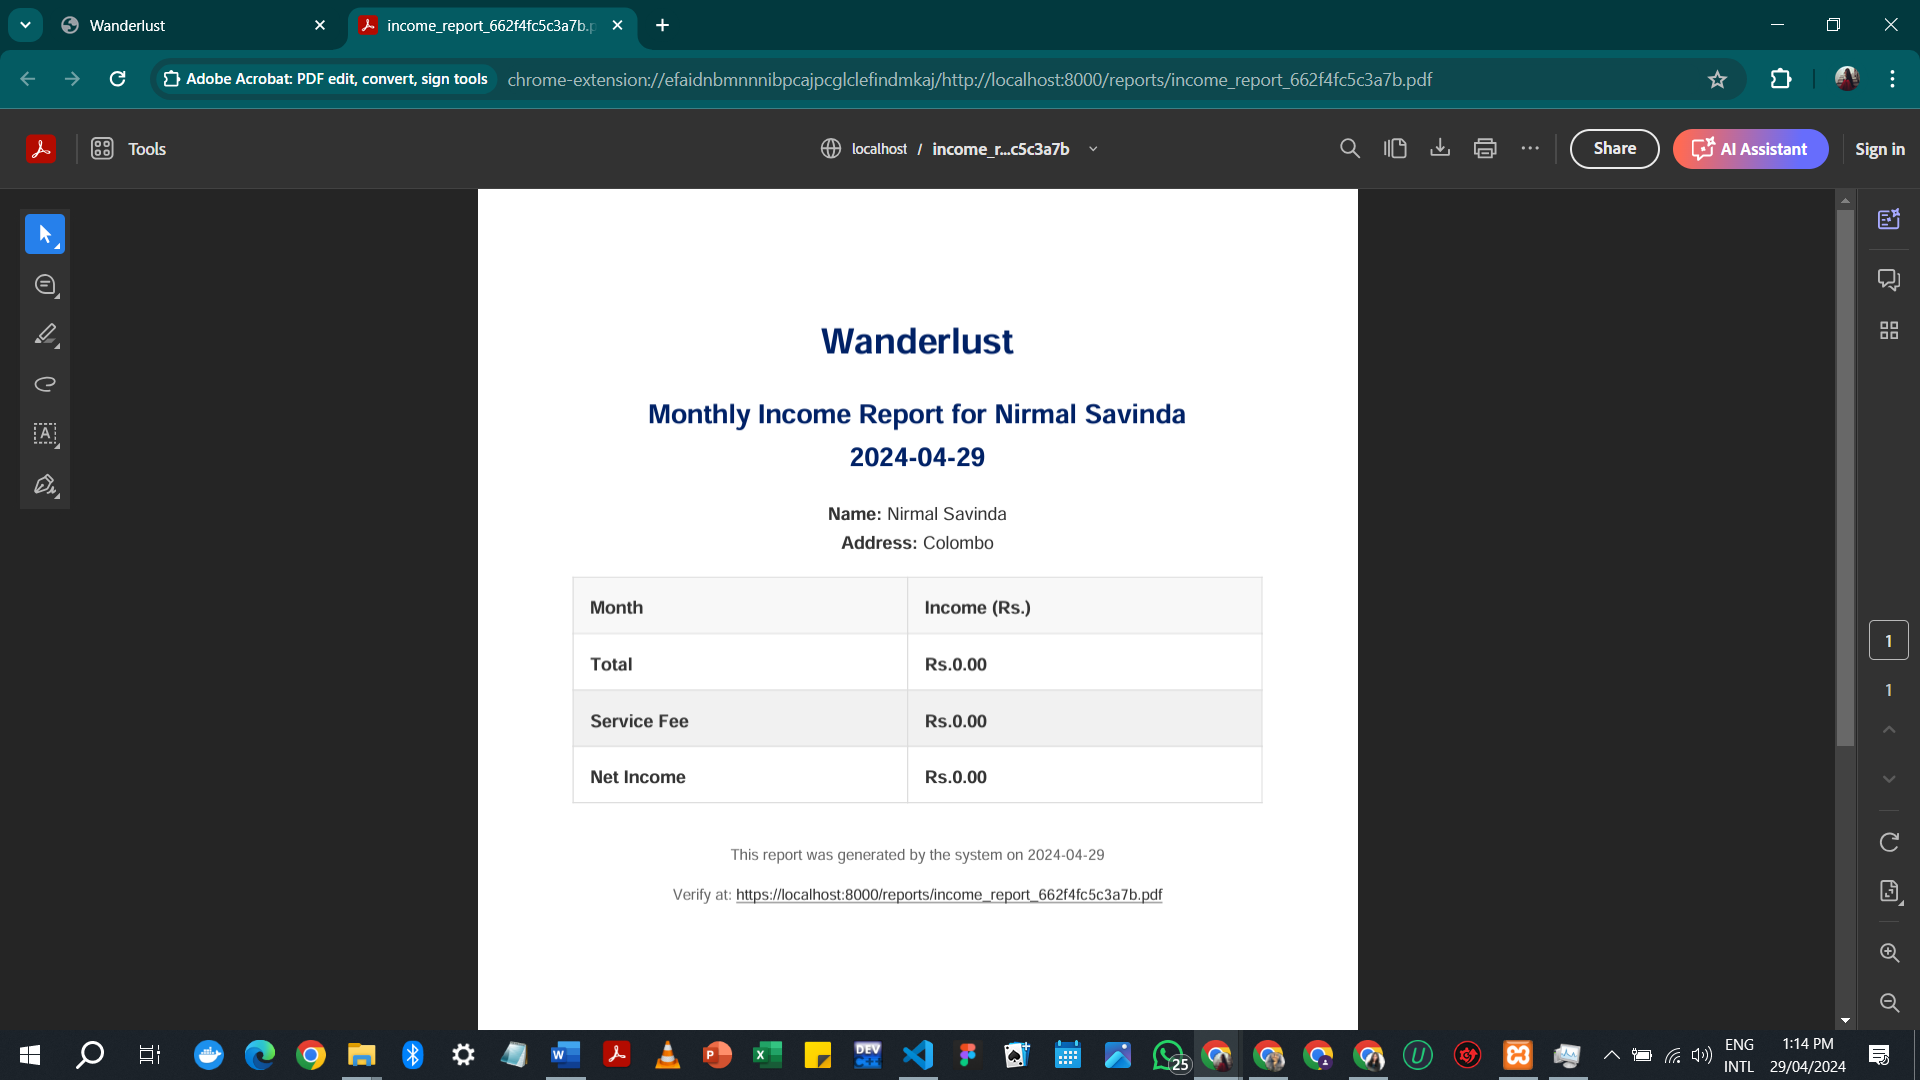
\includegraphics[width=1\textwidth]{Images/Test Cases/19. valid report.png}
\end{figure}
\clearpage


\textbf{Equipment Handling}\\
\begin{table}[ht]
\centering
\begin{tabularx}{\textwidth}{|c|c|X|X|X|c|}
\hline
\textbf{TID} & \textbf{User Role} & \textbf{Scenario Description} & \textbf{Steps to Execute} & \textbf{Expected Result} & \textbf{Status} \\ \hline
20 & Rental Services & Valid Equipment adding & 1.Click 'Add new' \newline2.Input valid data for the fields \newline3.Click 'Add equipment' & Equipment is added successfully & Pass \\ \hline
\end{tabularx}
\caption{Valid equipment added}
\end{table}

\begin{figure}[h!]
    \centering
    \textbf{Actual Result}
    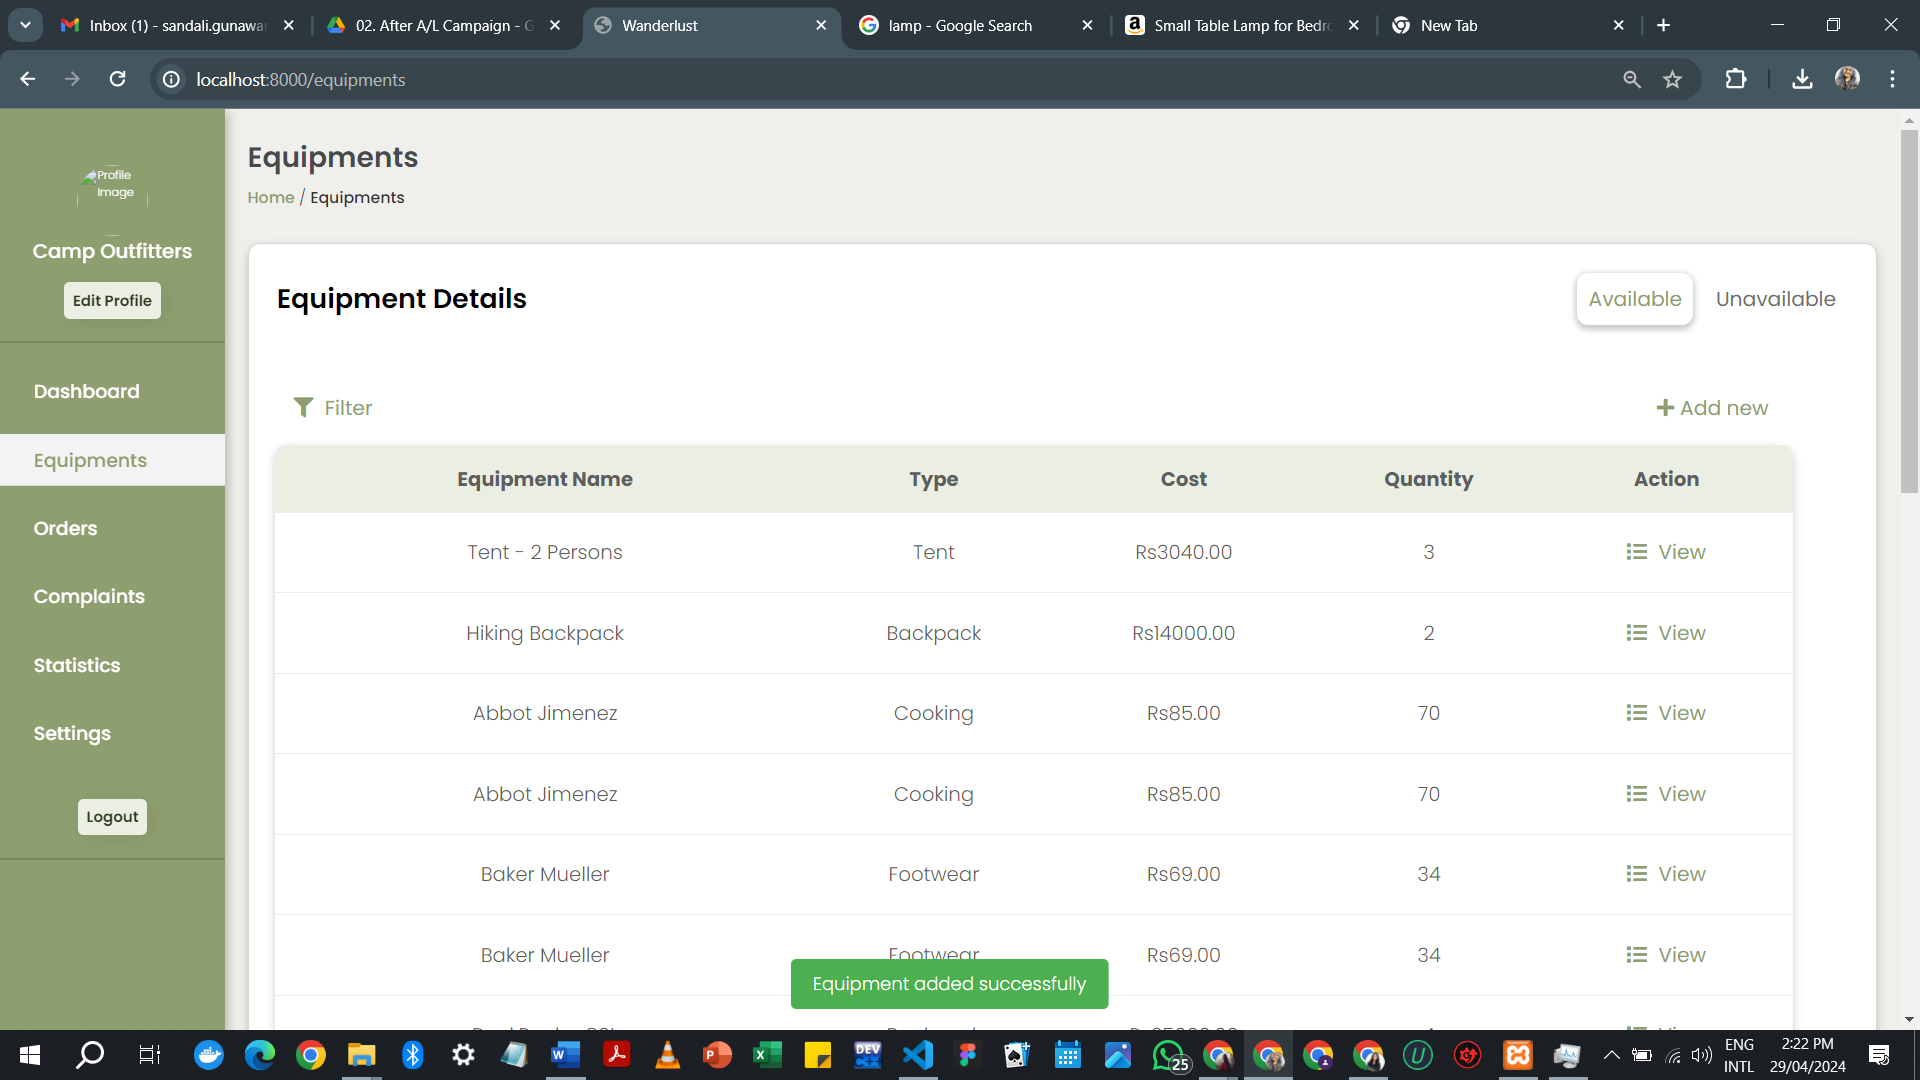
\includegraphics[width=1\textwidth]{Images/Test Cases/20. Valid Equipment adding.png}
\end{figure}
\clearpage


\begin{table}[ht]
\centering
\begin{tabularx}{\textwidth}{|c|c|X|X|X|c|}
\hline
\textbf{TID} & \textbf{User Role} & \textbf{Scenario Description} & \textbf{Steps to Execute} & \textbf{Expected Result} & \textbf{Status} \\ \hline
21 & Rental Services & Invalid Equipment adding & 1.Click 'Add new' \newline2.Input invalid data (invalid name or negative count) \newline3.Click 'Add equipment' & Error message pops & Pass \\ \hline
\end{tabularx}
\caption{Invalid equipment added}
\end{table}

\begin{figure}[h!]
    \centering
    \textbf{Actual Result}
    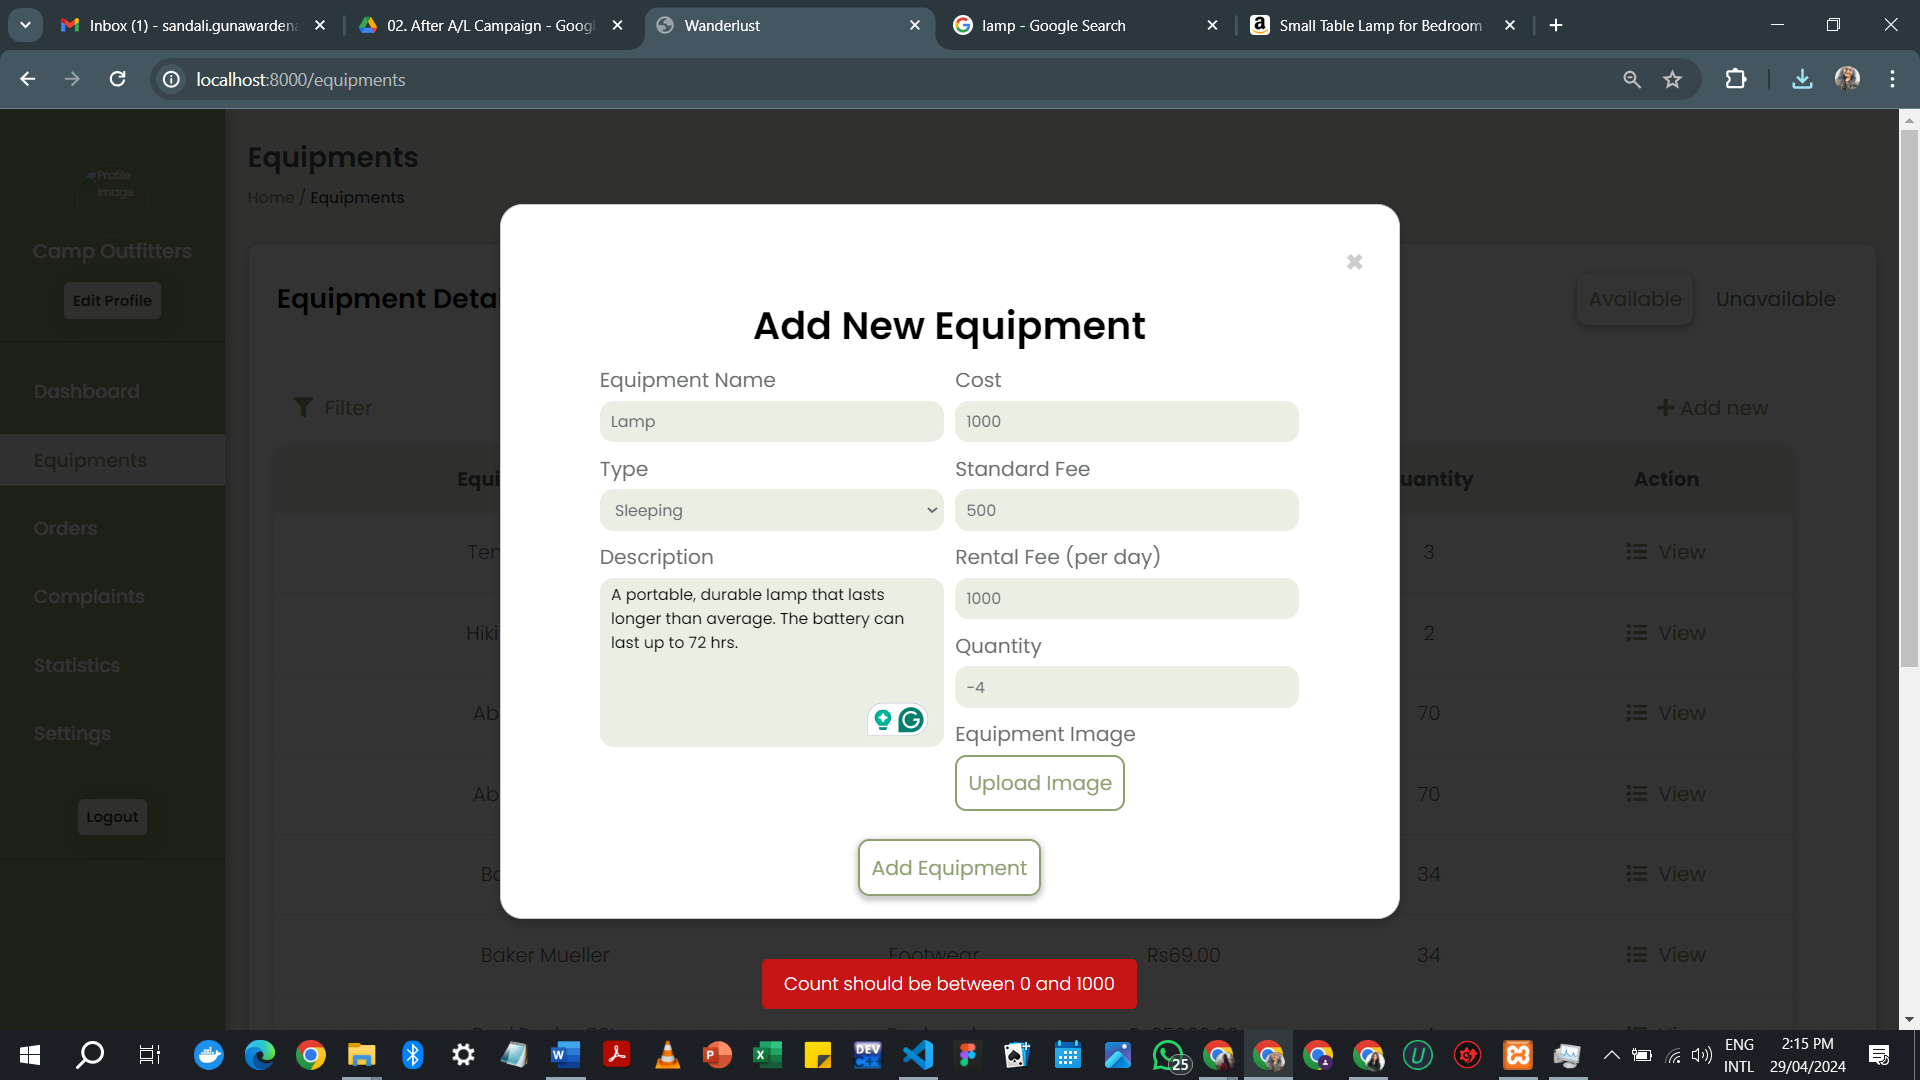
\includegraphics[width=1\textwidth]{Images/Test Cases/21. Invalid Equipment adding.png}
\end{figure}
\clearpage


\begin{table}[ht]
\centering
\begin{tabularx}{\textwidth}{|c|c|X|X|X|c|}
\hline
\textbf{TID} & \textbf{User Role} & \textbf{Scenario Description} & \textbf{Steps to Execute} & \textbf{Expected Result} & \textbf{Status} \\ \hline
21 & Rental Services & Invalid Equipment adding & 1.Click 'Add new' \newline2.Input invalid data (invalid name or negative count) \newline3.Click 'Add equipment' & Error message pops & Pass \\ \hline
\end{tabularx}
\caption{Invalid equipment added}
\end{table}

\begin{figure}[h!]
    \centering
    \textbf{Actual Result}
    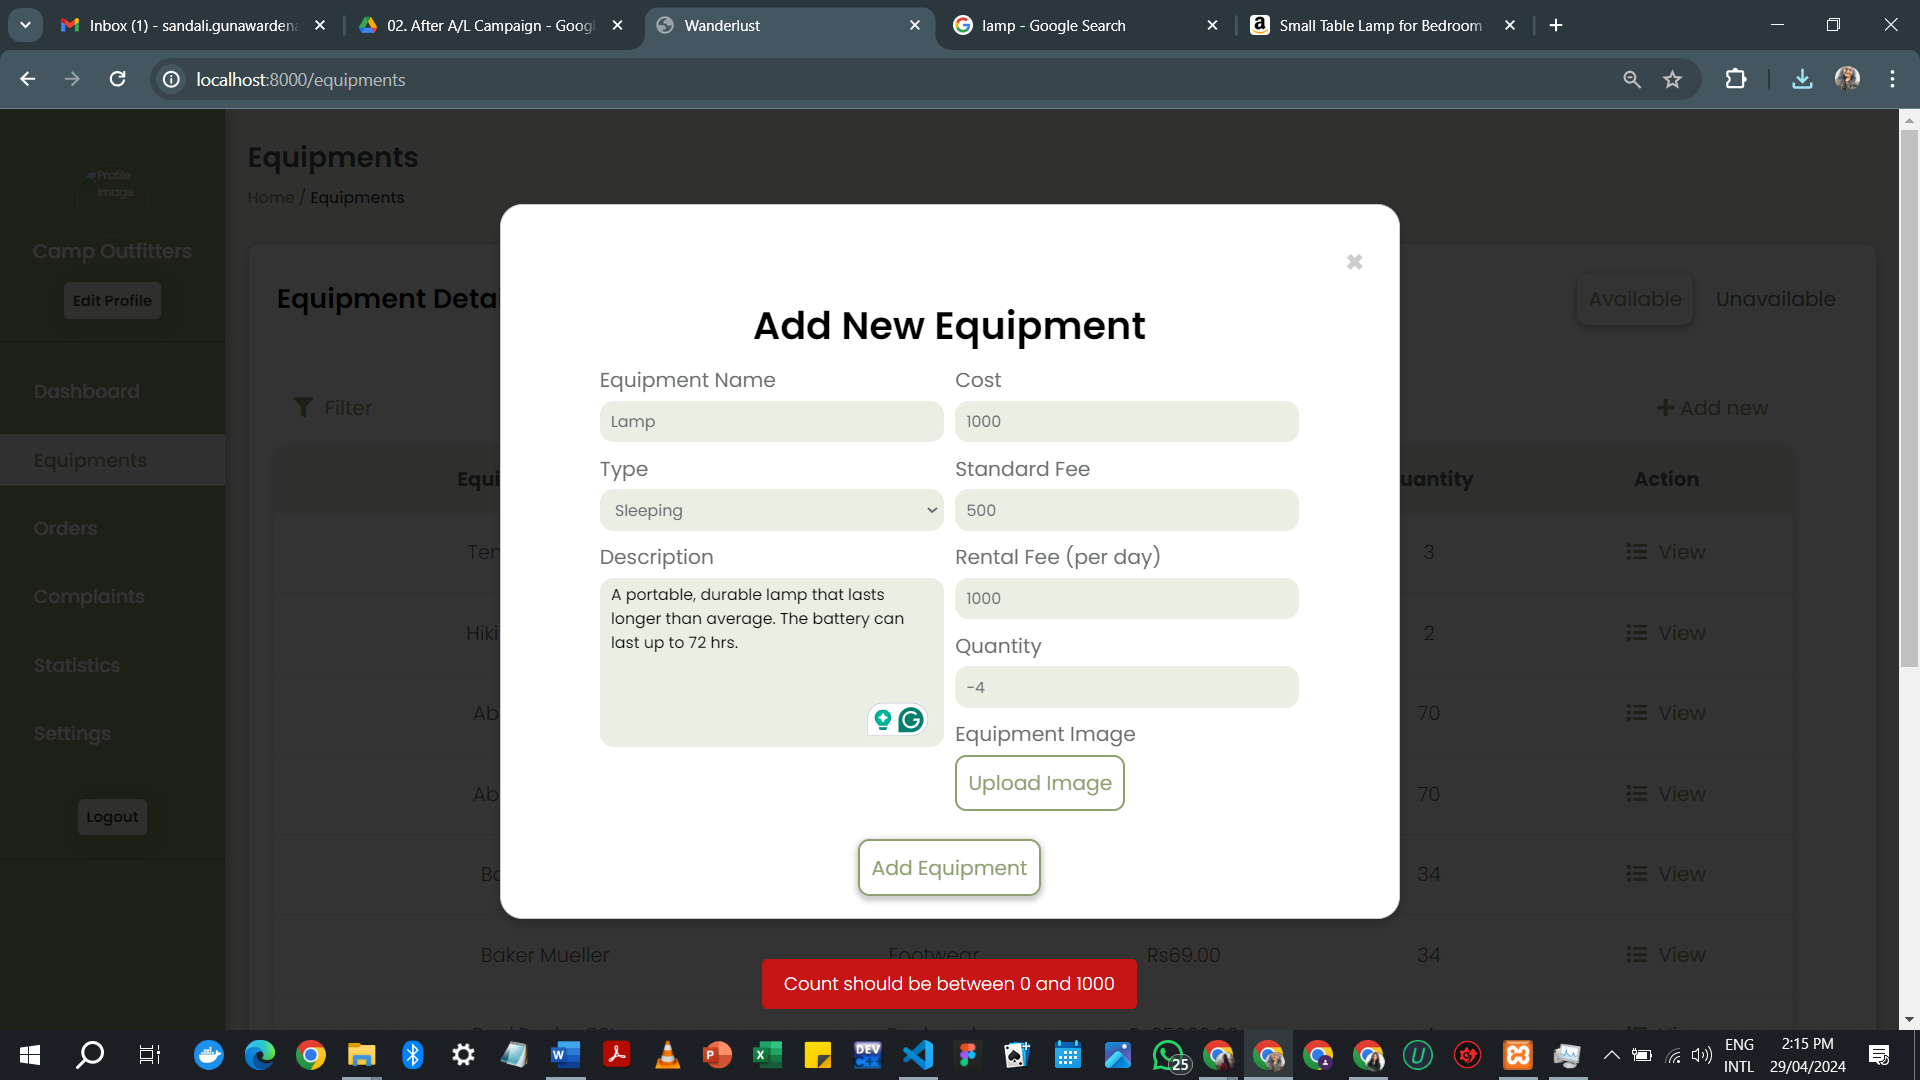
\includegraphics[width=1\textwidth]{Images/Test Cases/21. Invalid Equipment adding.png}
\end{figure}
\clearpage



\begin{table}[ht]
\centering
\begin{tabularx}{\textwidth}{|c|c|X|X|X|c|}
\hline
\textbf{TID} & \textbf{User Role} & \textbf{Scenario Description} & \textbf{Steps to Execute} & \textbf{Expected Result} & \textbf{Status} \\ \hline
22 & Rental Services & Equipment deleting & 1.Click 'View' \newline2.Select 'Delete' \newline3. Confirm deletion & Equipment is deleted & Pass \\ \hline
\end{tabularx}
\caption{Equipment deleting}
\end{table}

\begin{figure}[h!]
    \centering
    \textbf{Actual Result}
    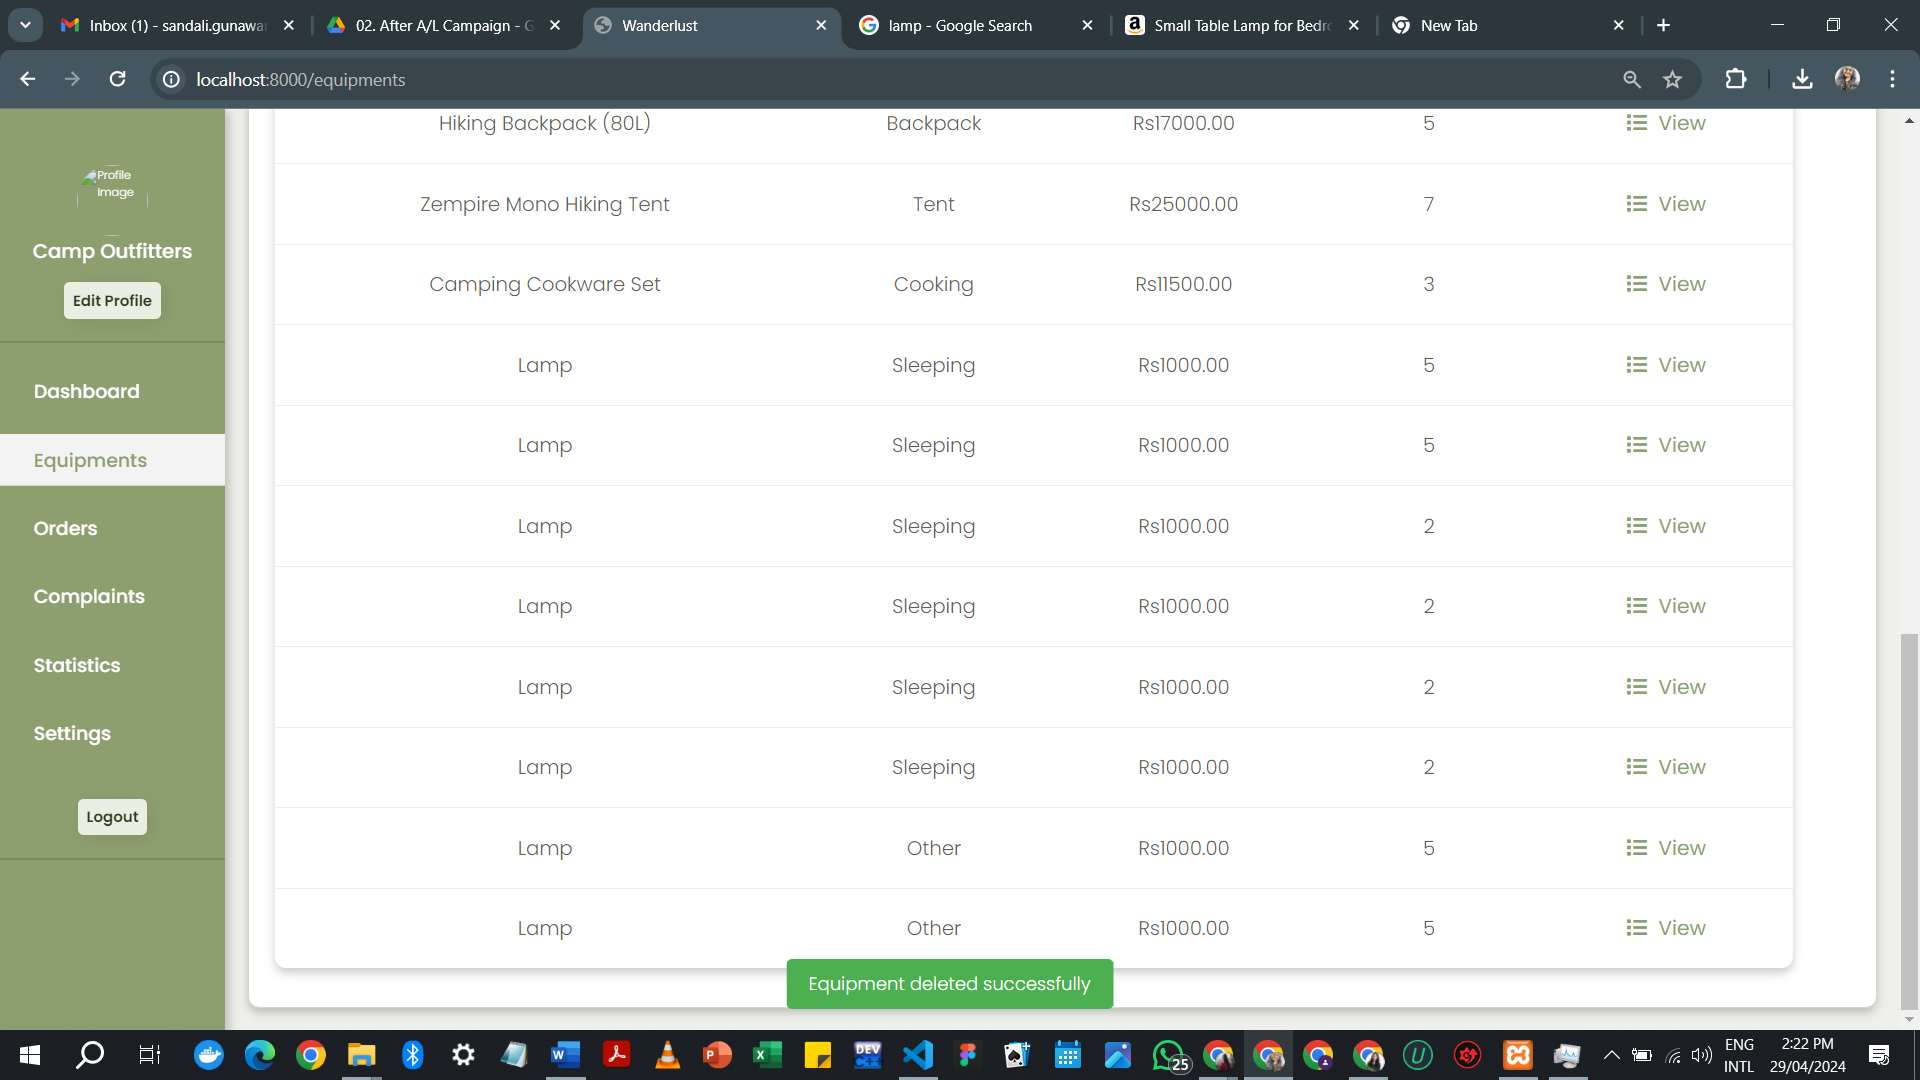
\includegraphics[width=1\textwidth]{Images/Test Cases/22. Equipment deleting.png}
\end{figure}
\clearpage


\begin{table}[ht]
\centering
\begin{tabularx}{\textwidth}{|c|c|X|X|X|c|}
\hline
\textbf{TID} & \textbf{User Role} & \textbf{Scenario Description} & \textbf{Steps to Execute} & \textbf{Expected Result} & \textbf{Status} \\ \hline
23 & Rental Services & Increase equipment count & 1.Click 'View' \newline2.Select 'Increase Quantity' \newline3. Confirm quantity & Equipment count is increases & Pass \\ \hline
\end{tabularx}
\caption{Increase equipment count}
\end{table}

\begin{figure}[h!]
    \centering
    \textbf{Actual Result}
    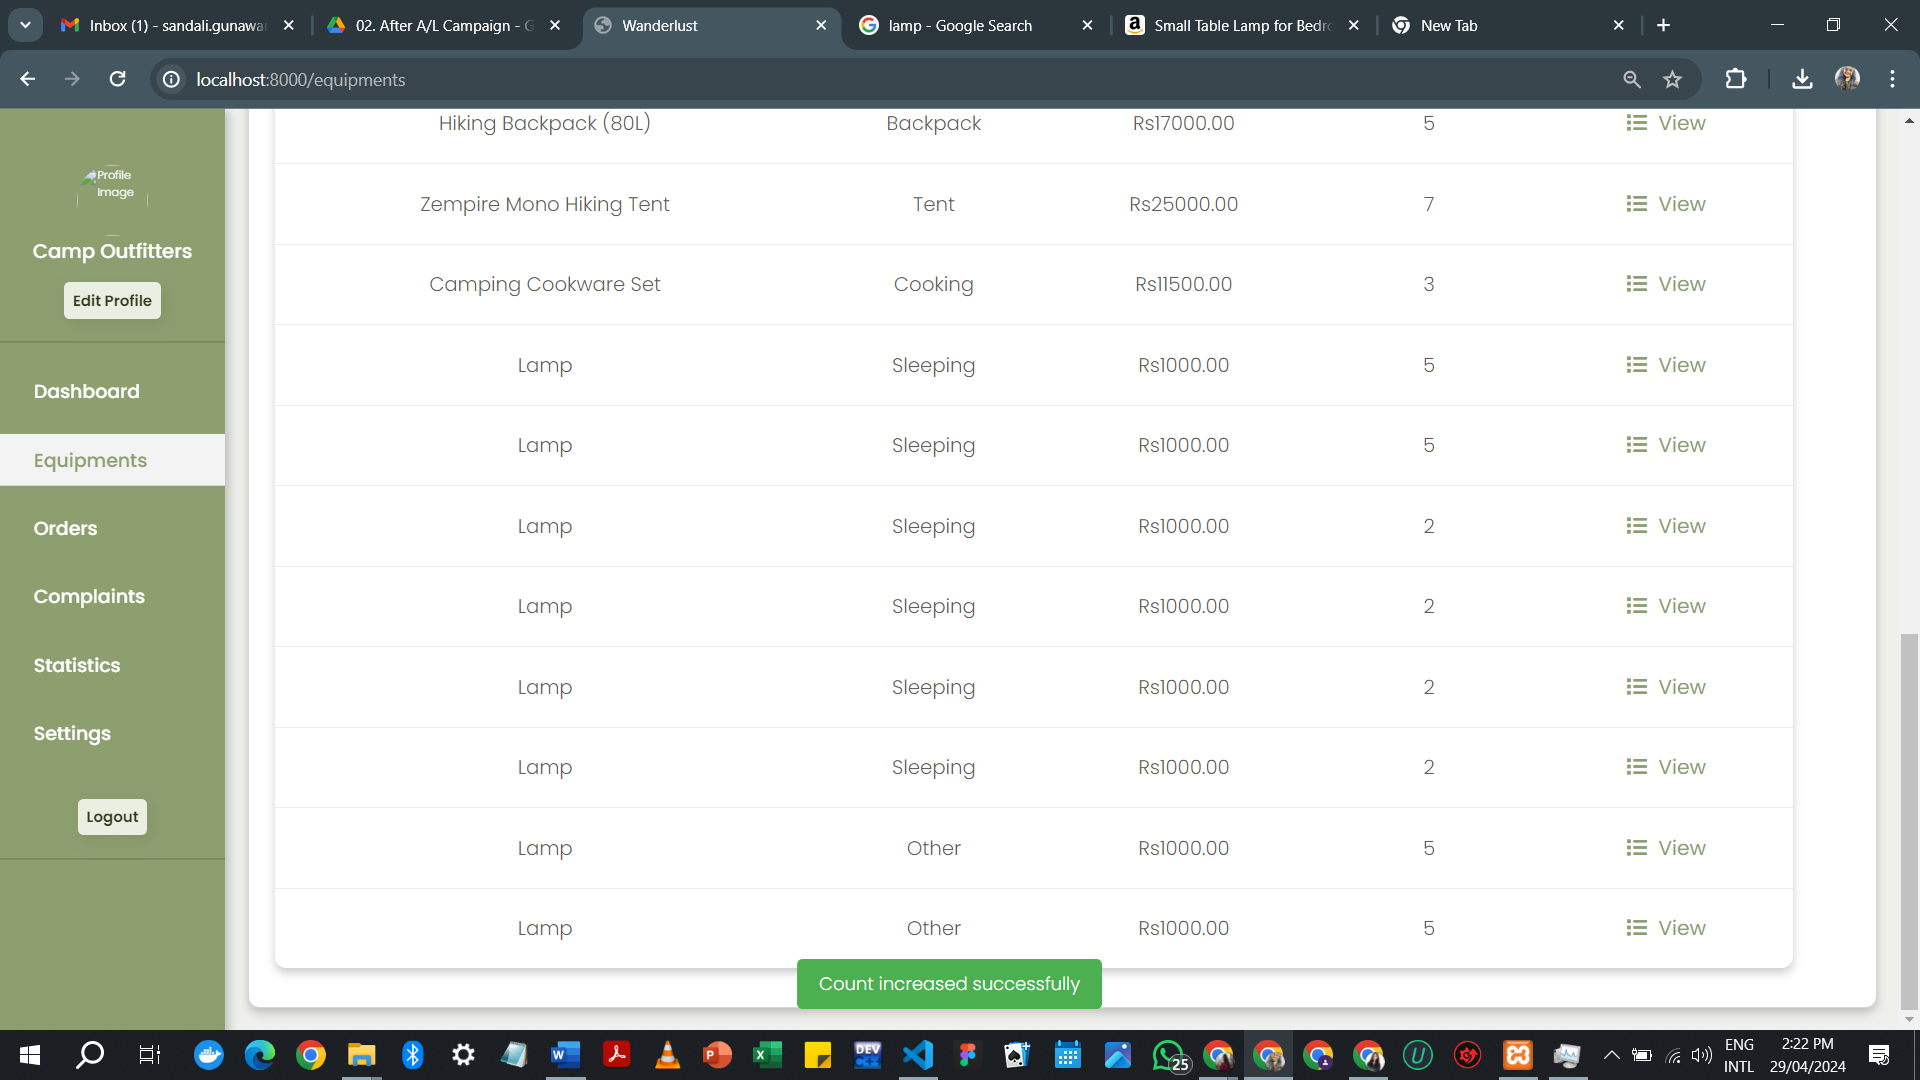
\includegraphics[width=1\textwidth]{Images/Test Cases/23. Increasing equipment count.png}
\end{figure}
\clearpage


\begin{table}[ht]
\centering
\begin{tabularx}{\textwidth}{|c|c|X|X|X|c|}
\hline
\textbf{TID} & \textbf{User Role} & \textbf{Scenario Description} & \textbf{Steps to Execute} & \textbf{Expected Result} & \textbf{Status} \\ \hline
    24 & Rental Services & Making equipment unavailable & 1.Click 'View' \newline2.Select 'Manage items' \newline3.Select 'Manage' icon of the relevant item \newline4.Select desired option & Equipment is made unavailable permanently/temporarily & Pass \\ \hline
\end{tabularx}
\caption{Making equipment unavailable}
\end{table}

\begin{figure}[h!]
    \centering
    \textbf{Actual Result}
    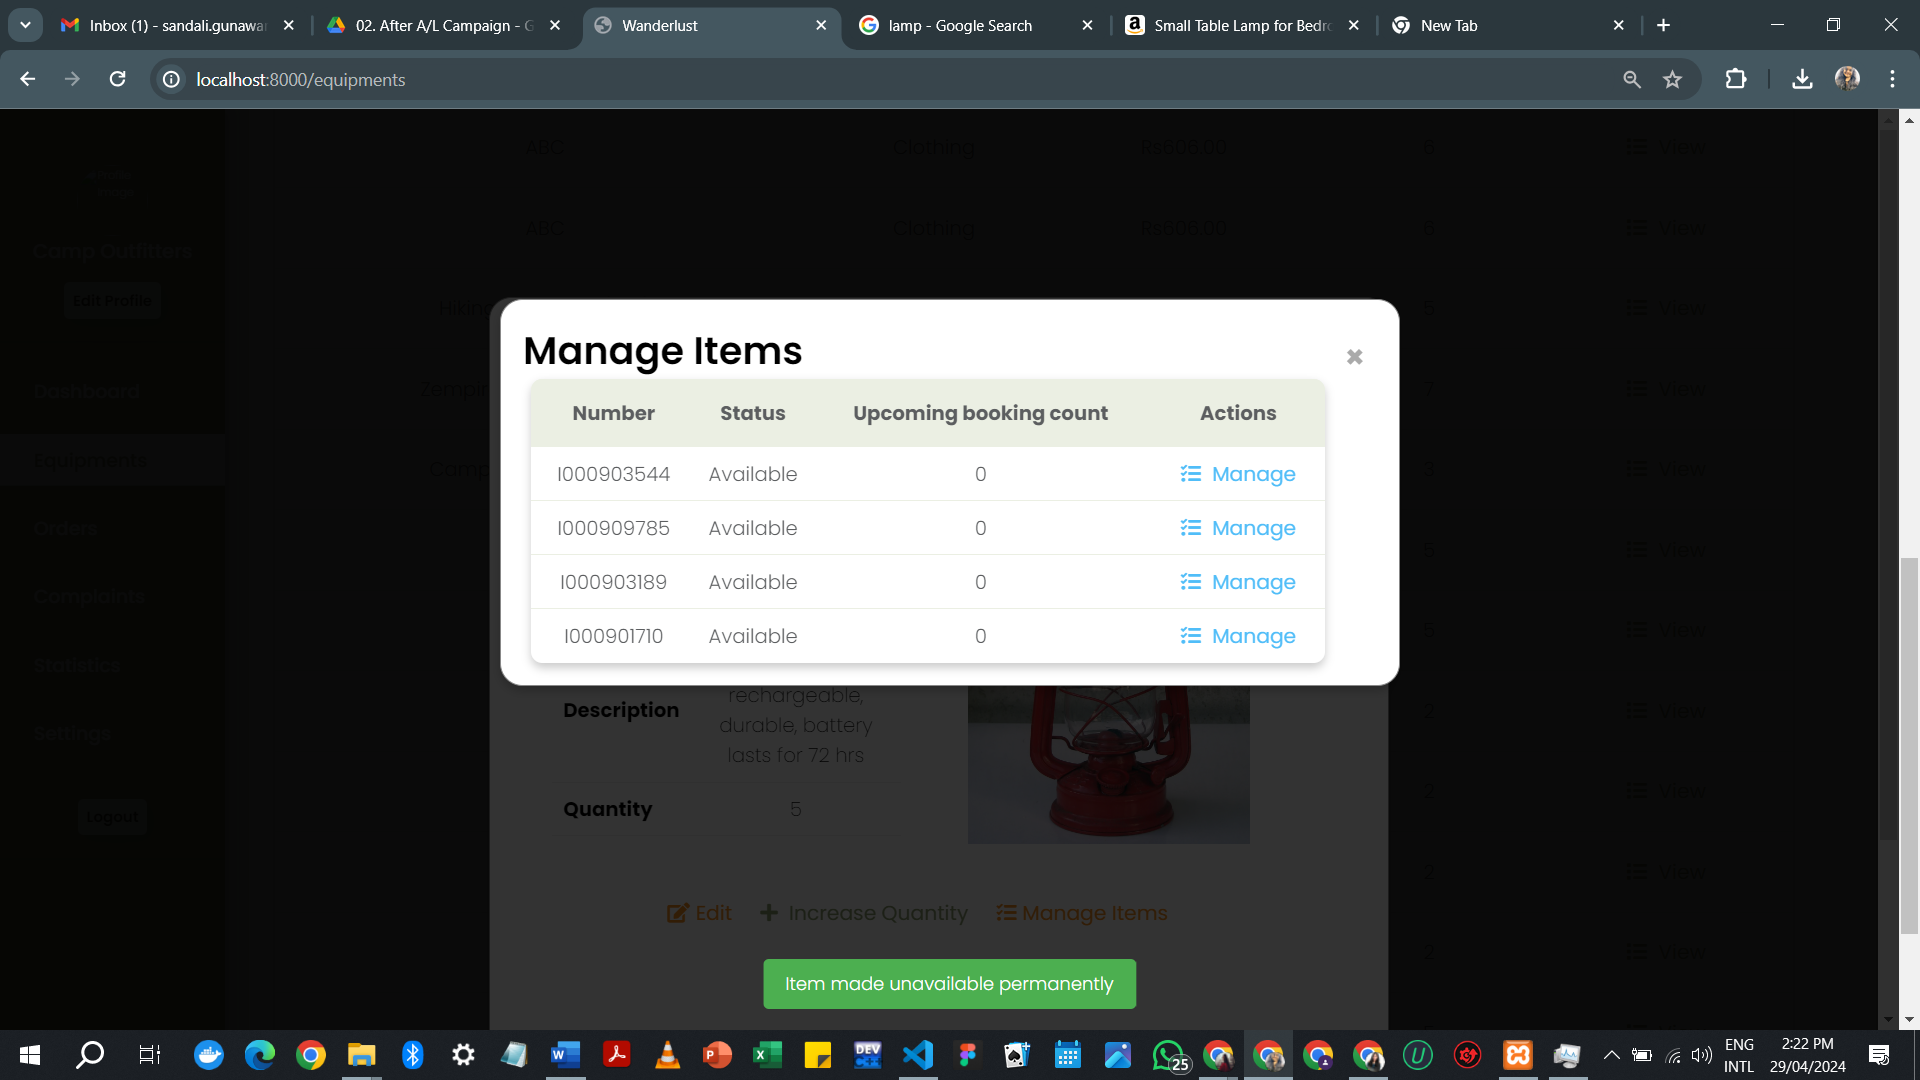
\includegraphics[width=1\textwidth]{Images/Test Cases/24. Making equipment temporarily unavailable.png}
\end{figure}
\clearpage


\textbf{Order Handling}\\
\begin{table}[ht]
\centering
\begin{tabularx}{\textwidth}{|c|c|X|X|X|c|}
\hline
\textbf{TID} & \textbf{User Role} & \textbf{Scenario Description} & \textbf{Steps to Execute} & \textbf{Expected Result} & \textbf{Status} \\ \hline
25 & Rental Services & Accepting/rejecting customer orders & 1.Click 'Orders' \newline2.Select 'Pending' \newline3.Select either 'Accept' or 'Reject' & Order status is updated in the customer's account & Pass \\ \hline
\end{tabularx}
\caption{Accepting/rejecting customer orders}
\end{table}

\begin{figure}[h!]
    \centering
    \textbf{Actual Result}
    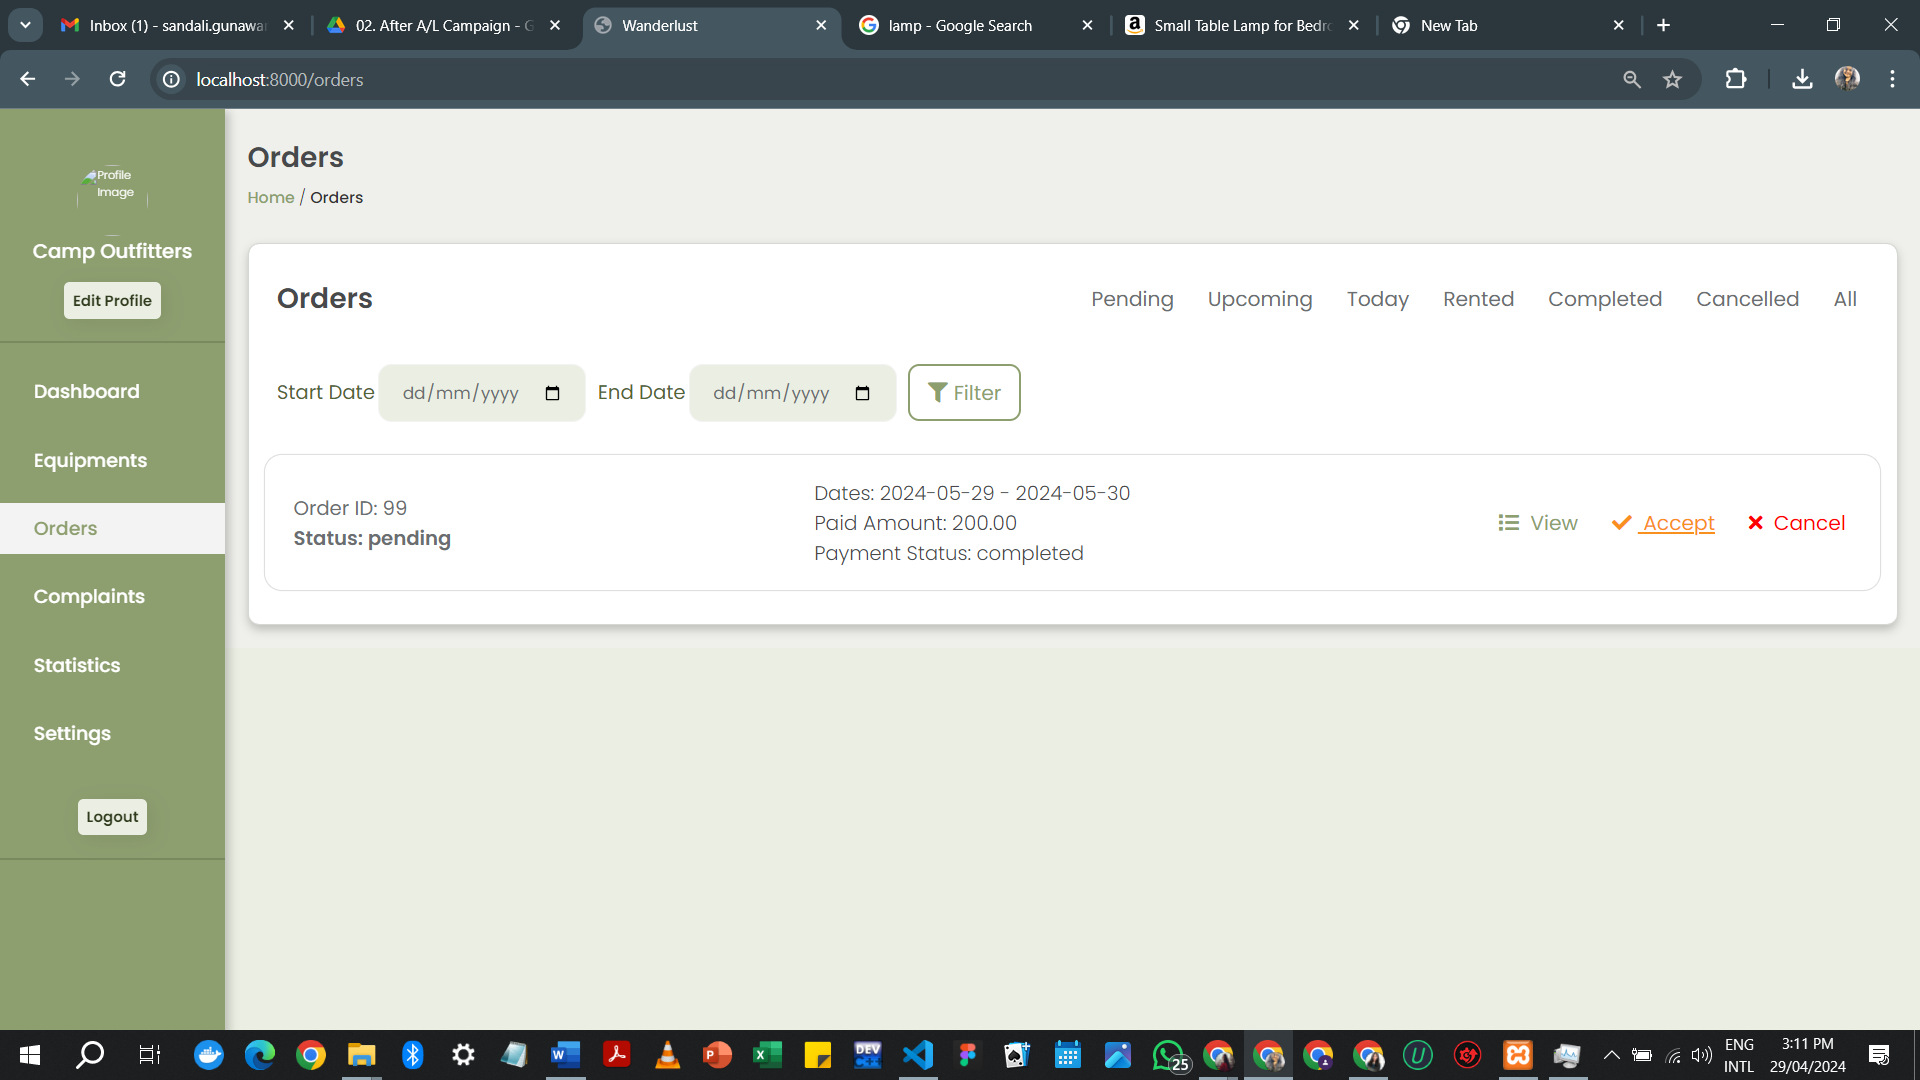
\includegraphics[width=1\textwidth]{Images/Test Cases/25. Accepting customer orders.png}
\end{figure}
\clearpage


\textbf{Complaint Handling}\\
\begin{table}[ht]
\centering
\begin{tabularx}{\textwidth}{|c|c|X|X|X|c|}
\hline
\textbf{TID} & \textbf{User Role} & \textbf{Scenario Description} & \textbf{Steps to Execute} & \textbf{Expected Result} & \textbf{Status} \\ \hline
26 & Rental Services & Complaint Handling & 1.Click 'Complaints' \newline2.Select 'Pending' \newline3.Select either 'Accept' or 'Reject' & Order status is updated accordingly in the customer's account and rental service's account & Pass \\ \hline
\end{tabularx}
\caption{Complaint Handling}
\end{table}

\begin{figure}[h!]
    \centering
    \textbf{Actual Result}
    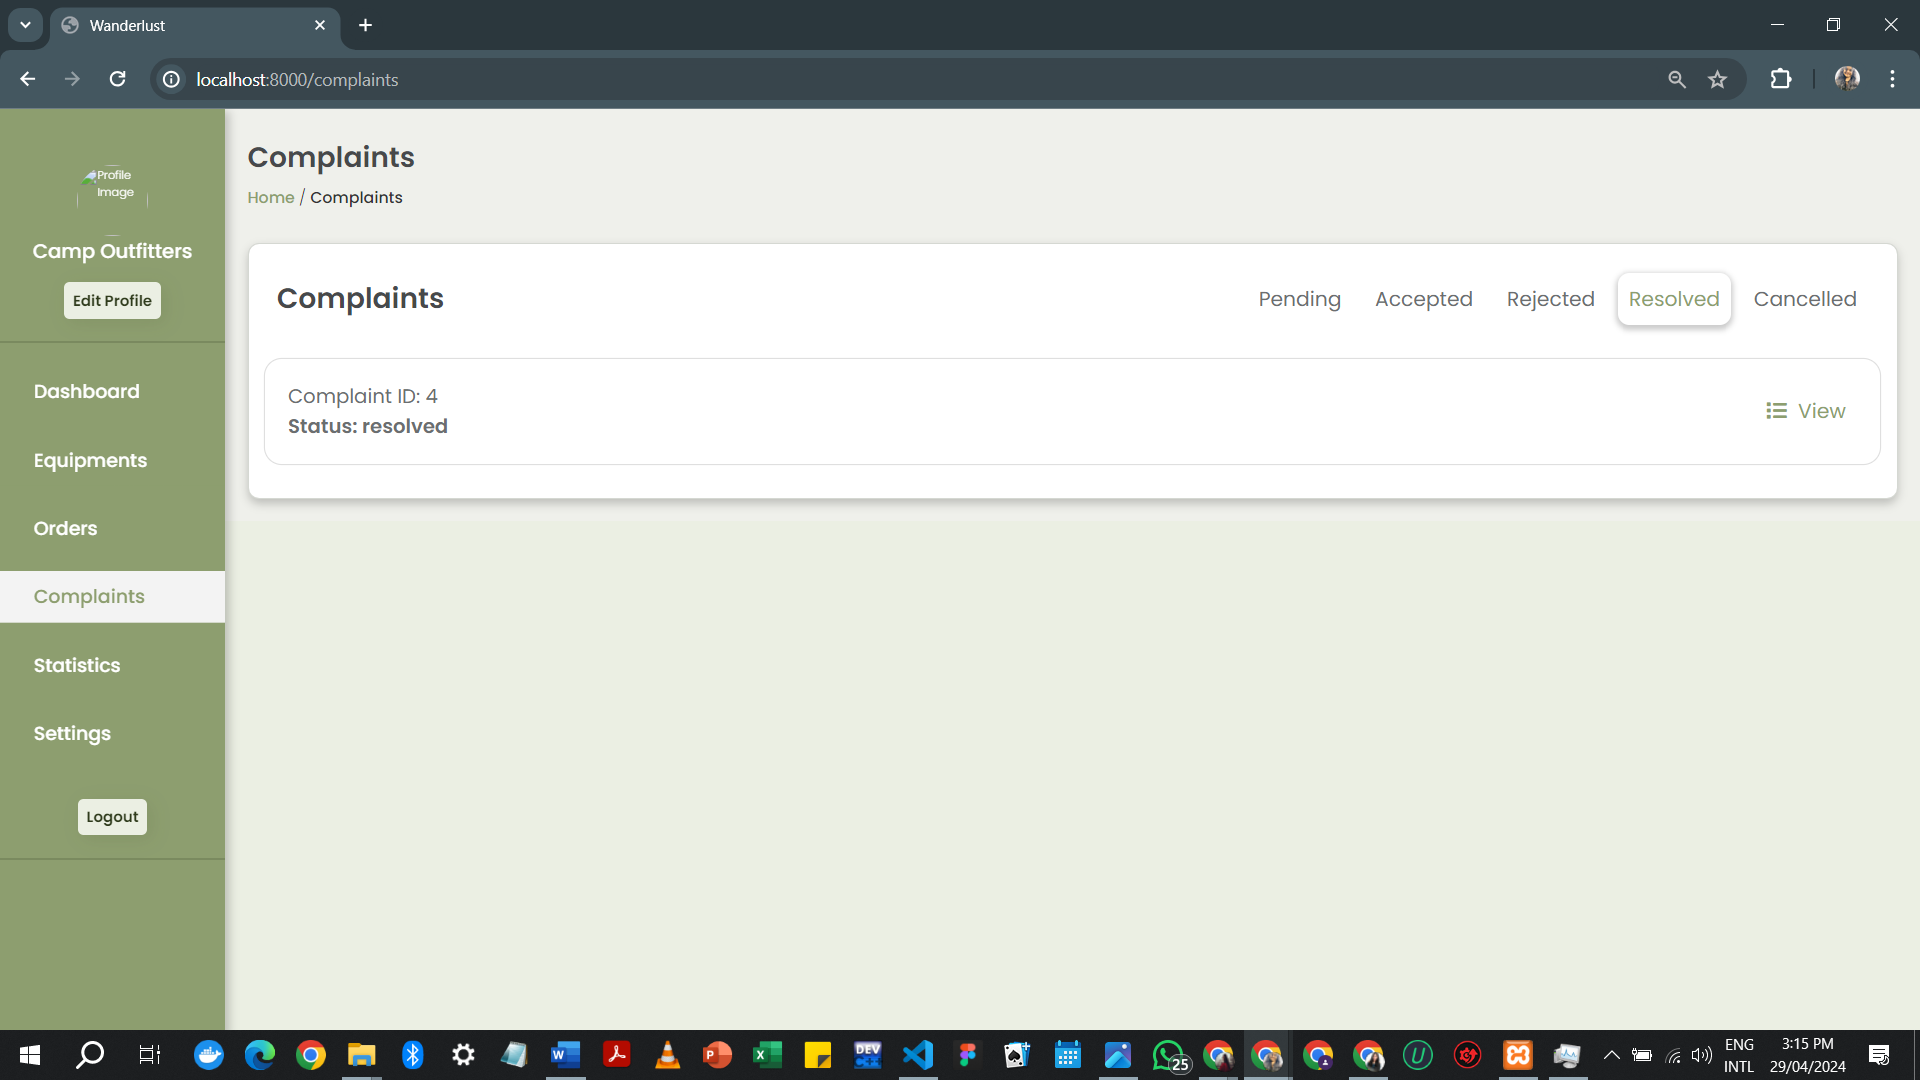
\includegraphics[width=1\textwidth]{Images/Test Cases/26. Complaints.png}
\end{figure}
\clearpage


\textbf{User Handling}\\
\begin{table}[ht]
\centering
\begin{tabularx}{\textwidth}{|c|c|X|X|X|c|}
\hline
\textbf{TID} & \textbf{User Role} & \textbf{Scenario Description} & \textbf{Steps to Execute} & \textbf{Expected Result} & \textbf{Status} \\ \hline
27 & Admin & User Handling - Rental Shops & 1.Select 'Rental Shops'\newline 2.Click 'View' of the specific Rental shop \newline3.Select 'Accept' or 'Reject' & User status is updated accordingly & Pass \\ \hline
\end{tabularx}
\caption{User Handling - Rental Shops}
\end{table}

\begin{figure}[h!]
    \centering
    \textbf{Actual Result}
    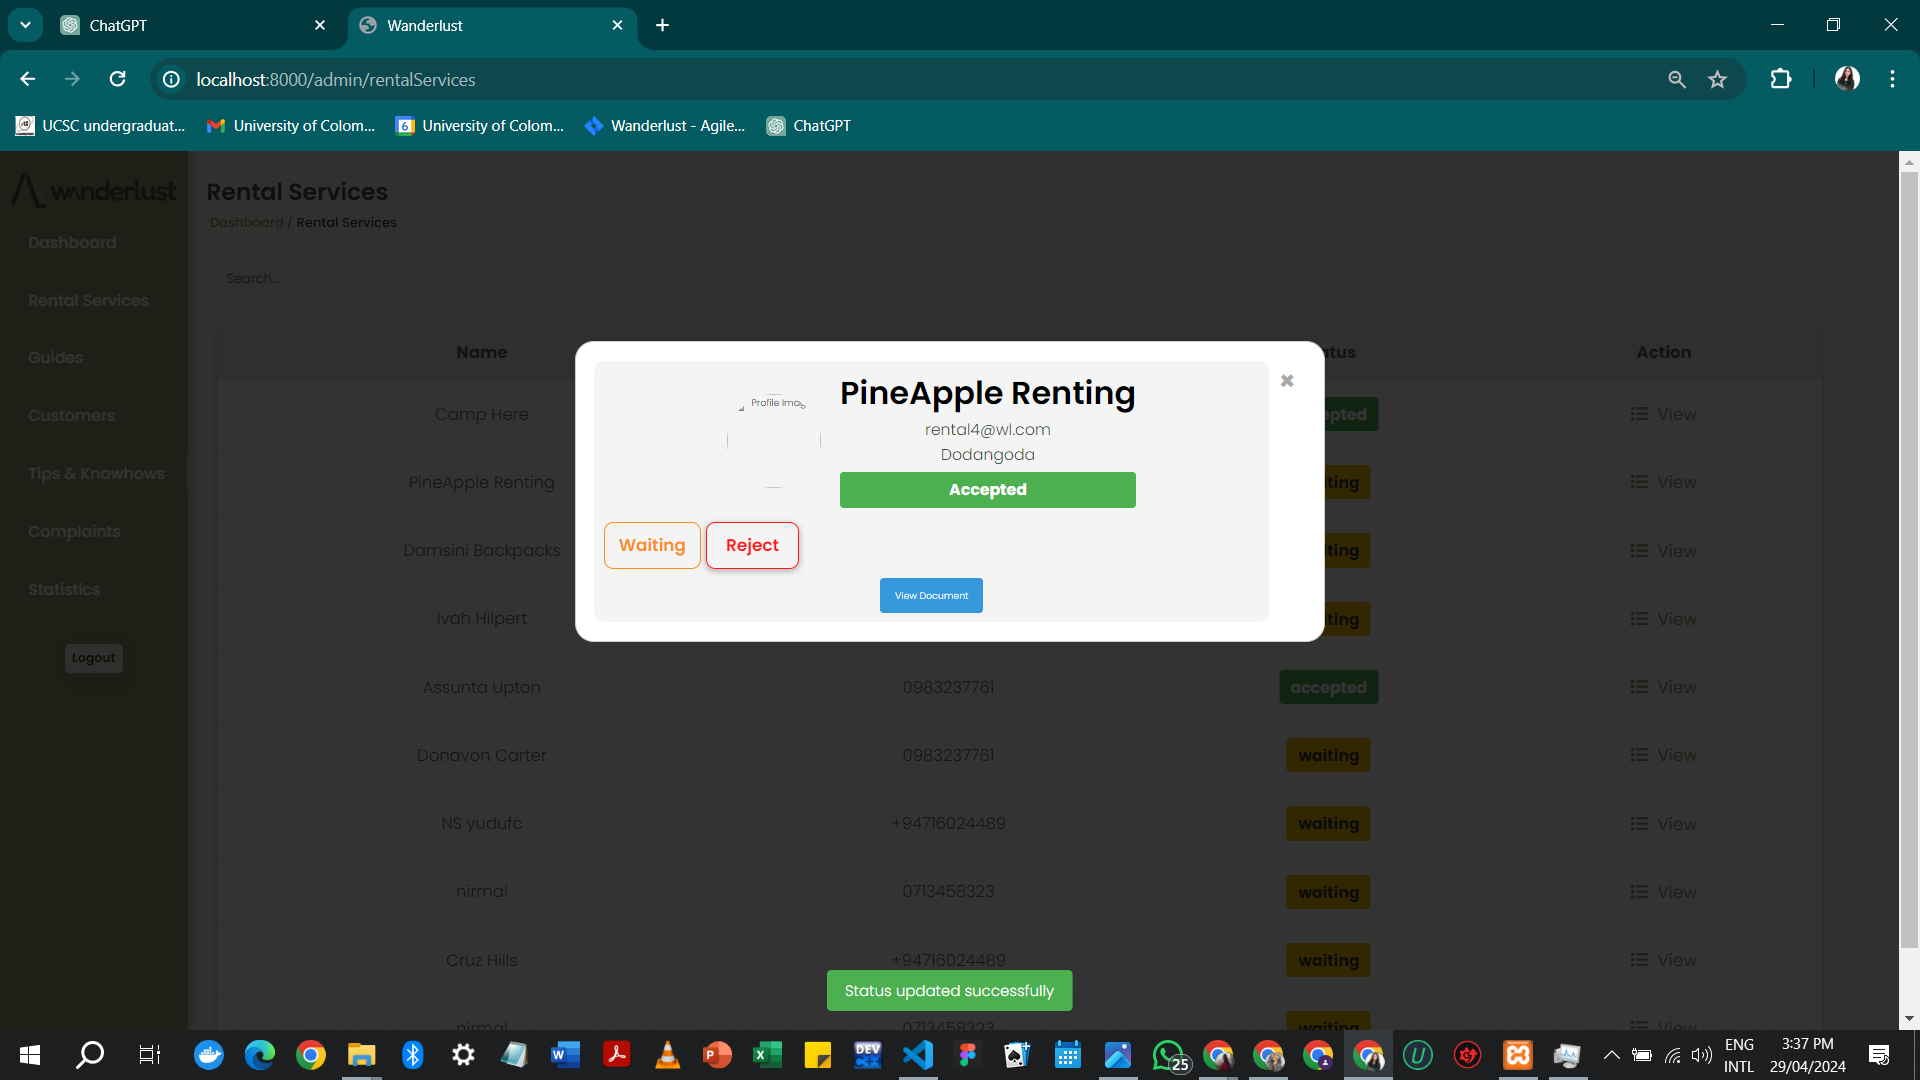
\includegraphics[width=1\textwidth]{Images/Test Cases/27. Handling Rentals.png}
\end{figure}
\clearpage


\begin{table}[ht]
\centering
\begin{tabularx}{\textwidth}{|c|c|X|X|X|c|}
\hline
\textbf{TID} & \textbf{User Role} & \textbf{Scenario Description} & \textbf{Steps to Execute} & \textbf{Expected Result} & \textbf{Status} \\ \hline
28 & Admin & User Handling - Guide &  1.Select 'Guides'\newline 2.Click 'View' of the specific Guide \newline3.Select 'Accept' or 'Reject' & User status is updated accordingly & Pass \\ \hline
\end{tabularx}
\caption{User Handling - Guides}
\end{table}

\begin{figure}[h!]
    \centering
    \textbf{Actual Result}
    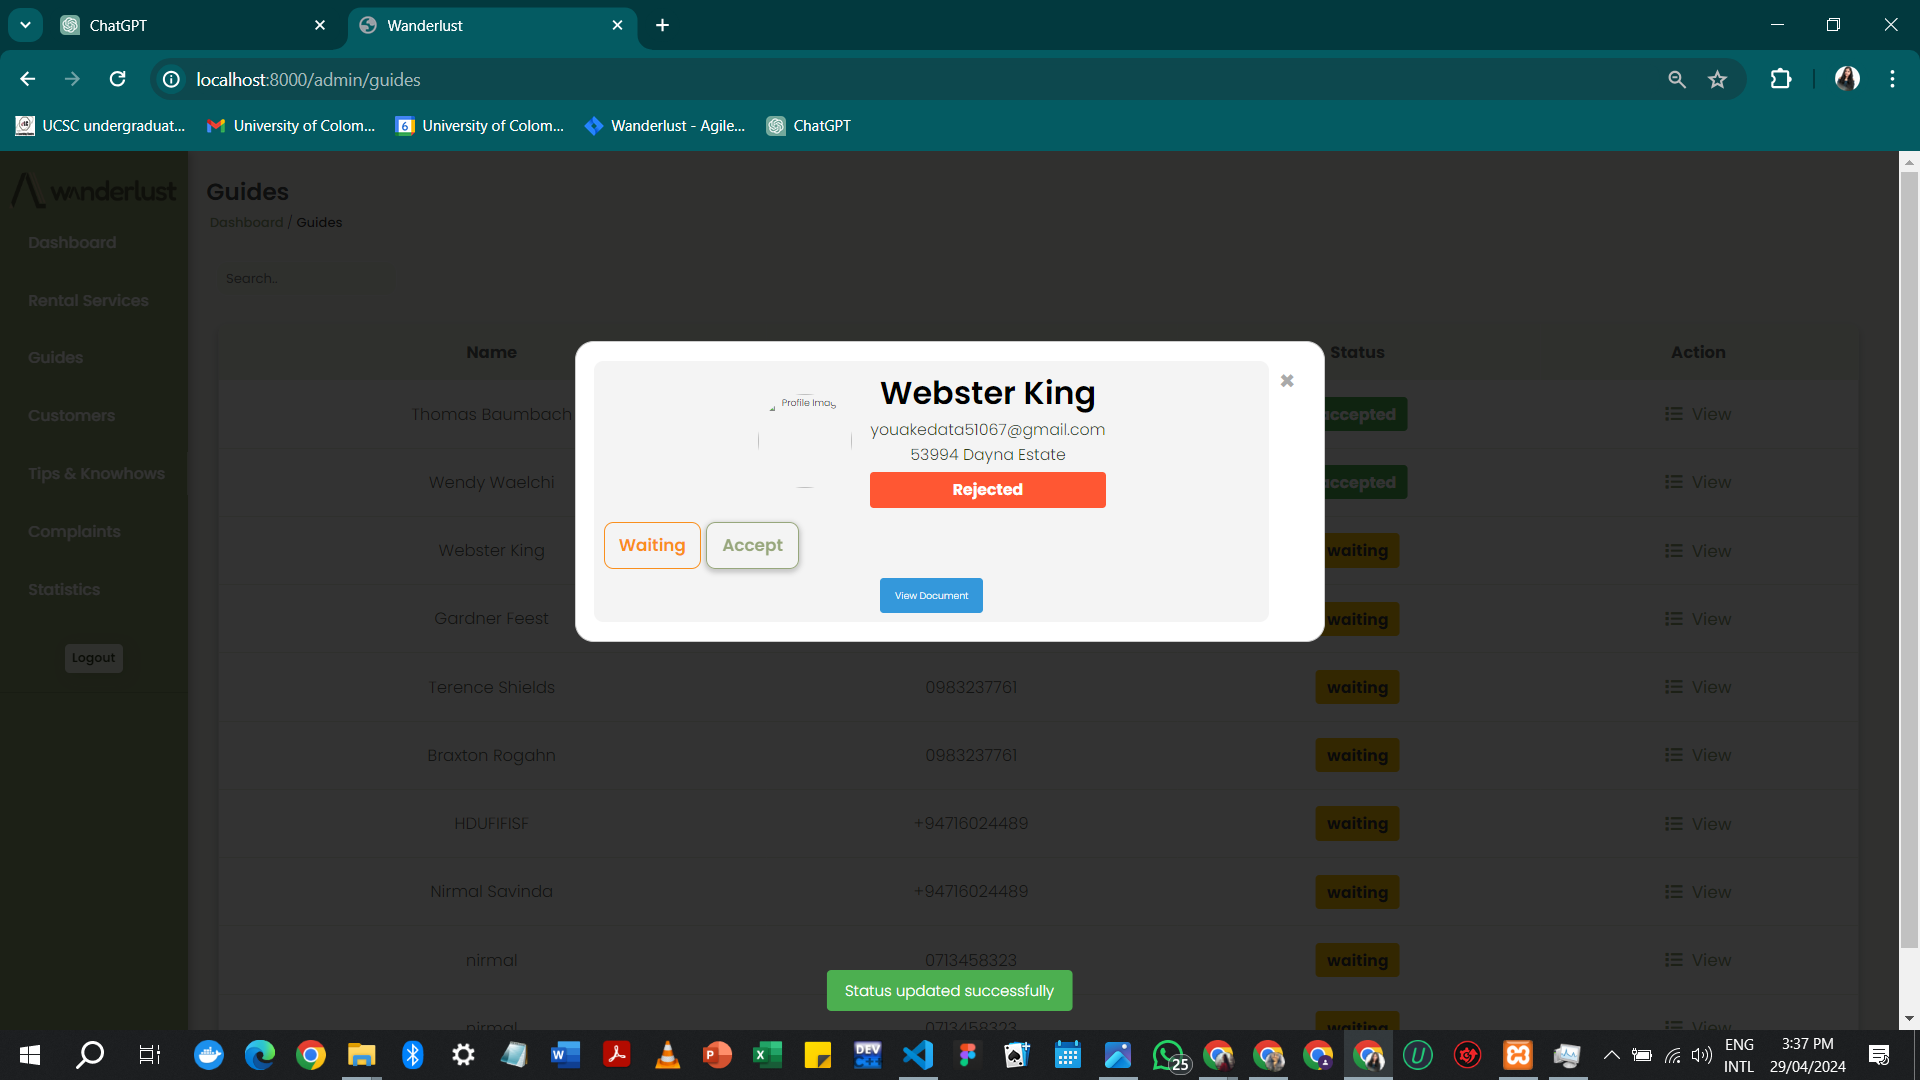
\includegraphics[width=1\textwidth]{Images/Test Cases/28. Handling Guides.png}
\end{figure}
\clearpage


\begin{table}[ht]
\centering
\begin{tabularx}{\textwidth}{|c|c|X|X|X|c|}
\hline
\textbf{TID} & \textbf{User Role} & \textbf{Scenario Description} & \textbf{Steps to Execute} & \textbf{Expected Result} & \textbf{Status} \\ \hline
29 & Admin & Resolving Complaints &  1.Select 'Complaints'\newline 2.Click the relevant user \newline3.Select 'Resolve' or 'Reject' & Complaint status is updated accordingly & Pass \\ \hline
\end{tabularx}
\caption{Resolving Complaints}
\end{table}

\begin{figure}[h!]
    \centering
    \textbf{Actual Result}
    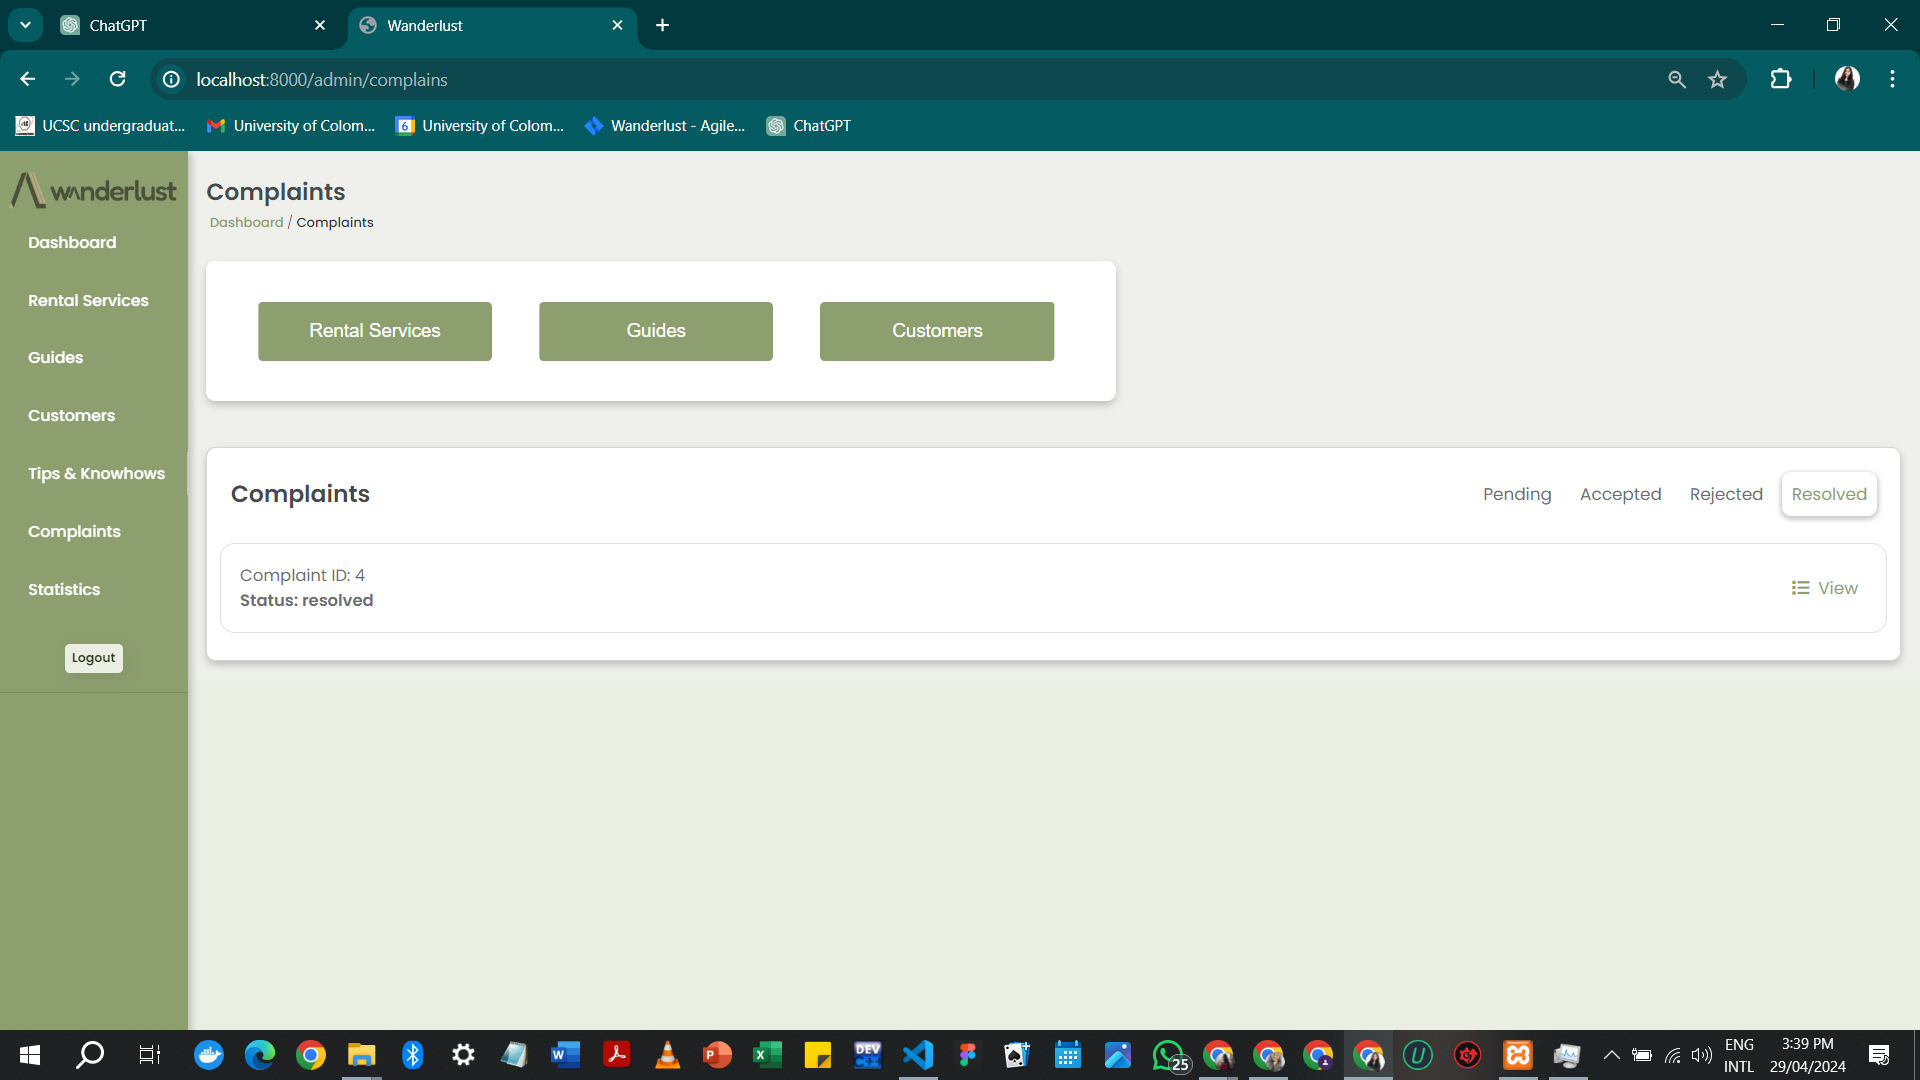
\includegraphics[width=1\textwidth]{Images/Test Cases/29. Resolving complaints.png}
\end{figure}
\clearpage
